\subsection{Question 1}

\begin{center}{\it Which face has a larger nose?}\end{center}

\begin{figure}[h]
\centering
\begin{subfigure}{0.4\textwidth}
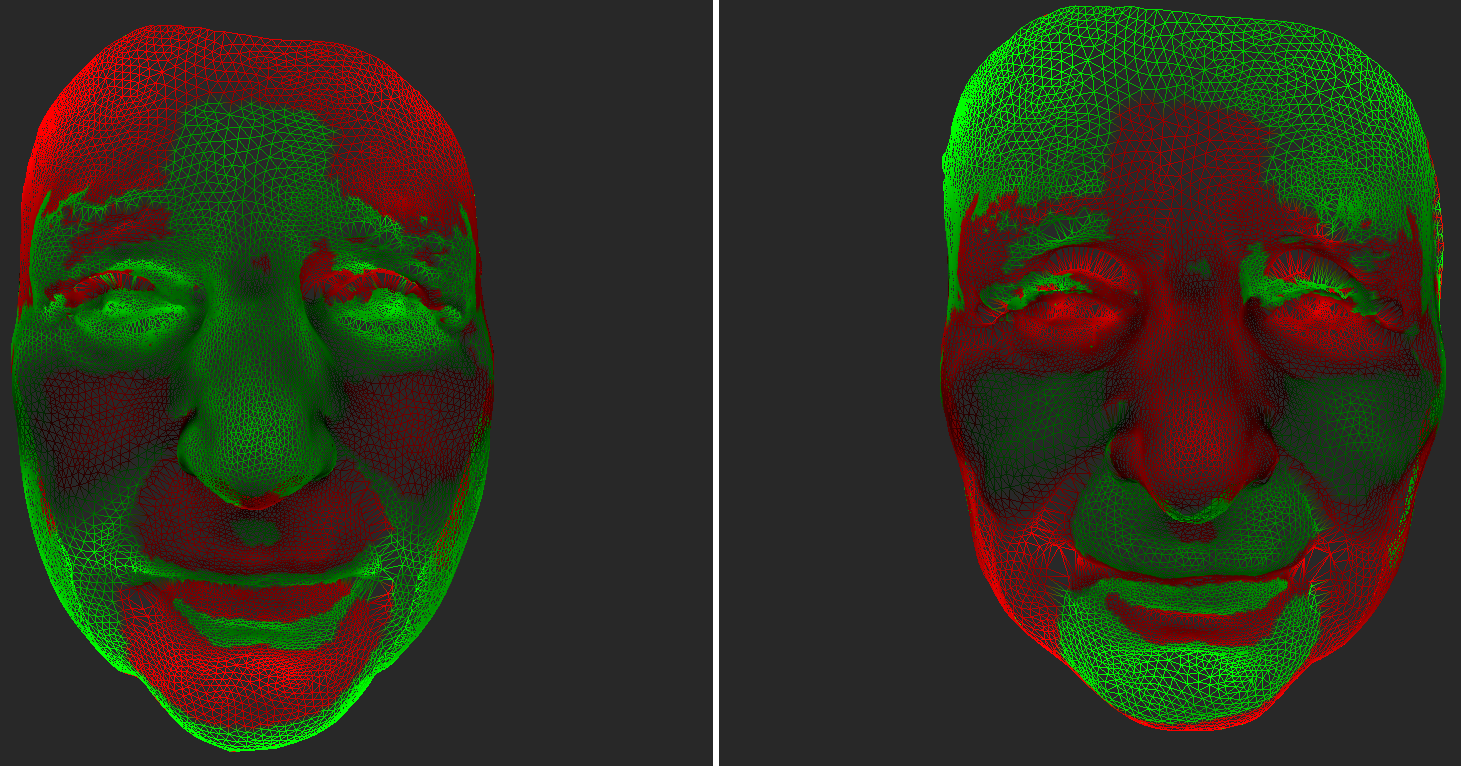
\includegraphics[width=\textwidth]{./screenshots/pair2.PNG}
\caption{}
\label{fig:0-2}
\end{subfigure}
\quad
\begin{subfigure}{0.4\textwidth}
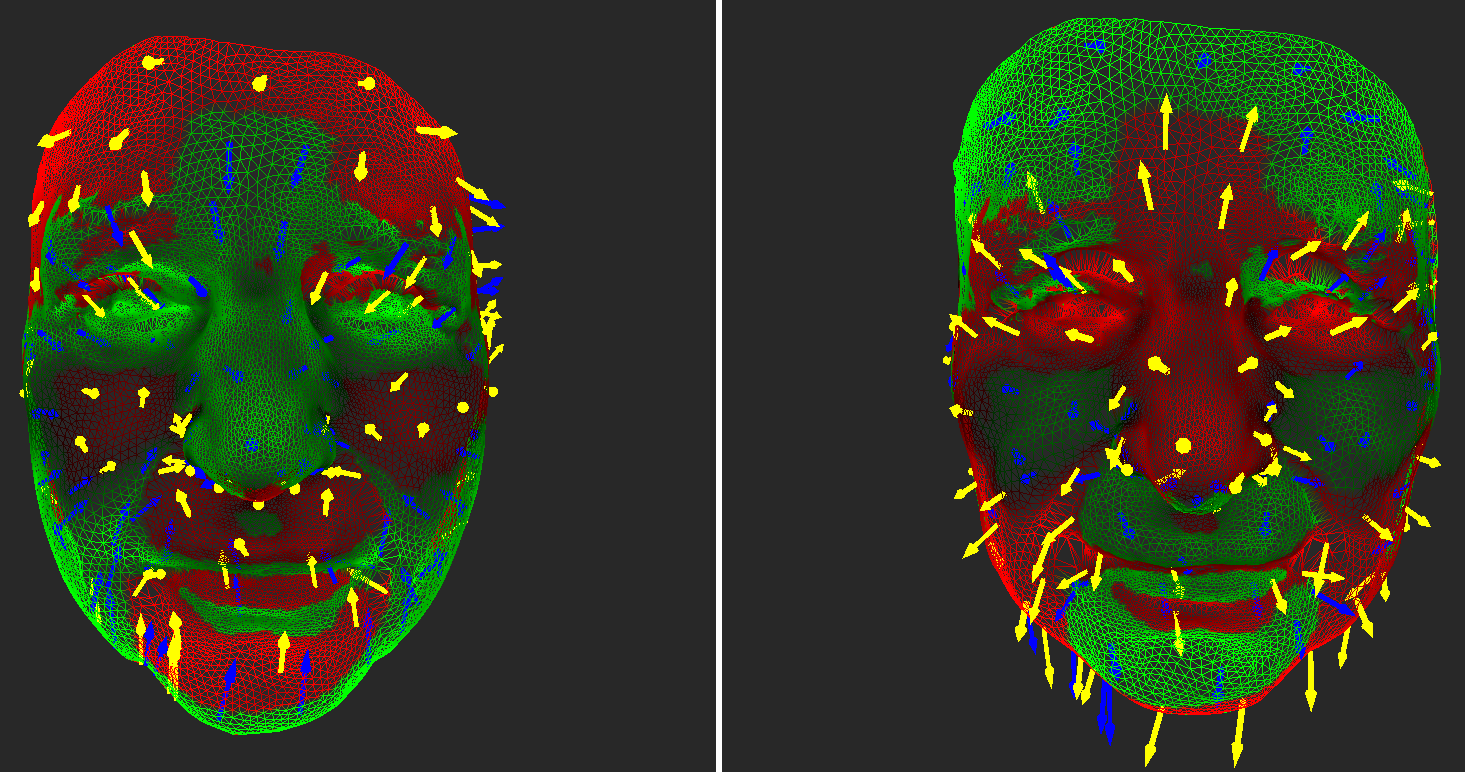
\includegraphics[width=\textwidth]{./screenshots/pair4.PNG}
\caption{}
\label{fig:0-4}
\end{subfigure}

\begin{subfigure}{0.4\textwidth}
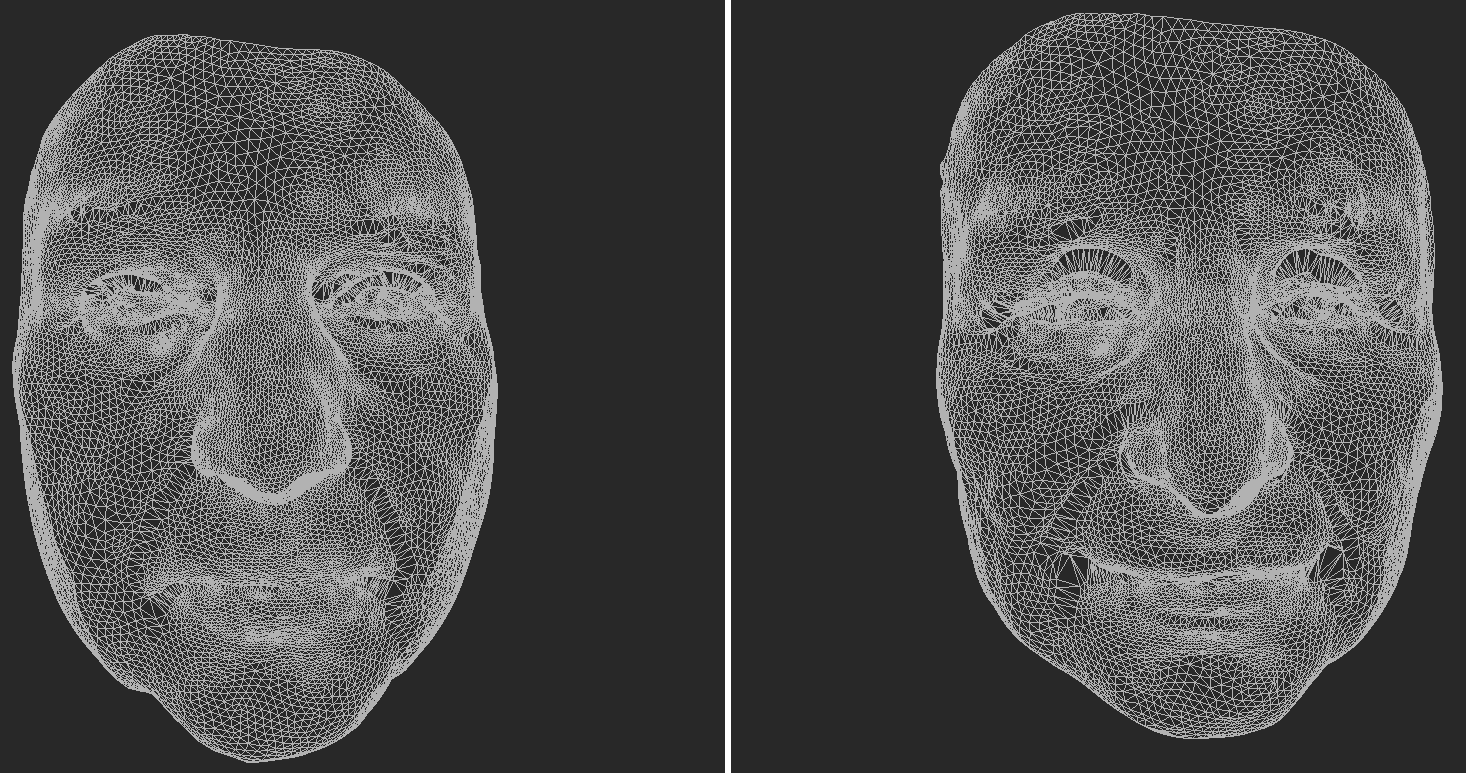
\includegraphics[width=\textwidth]{./screenshots/pair1.PNG}
\caption{}
\label{fig:0-1}
\end{subfigure}
\quad
\begin{subfigure}{0.4\textwidth}
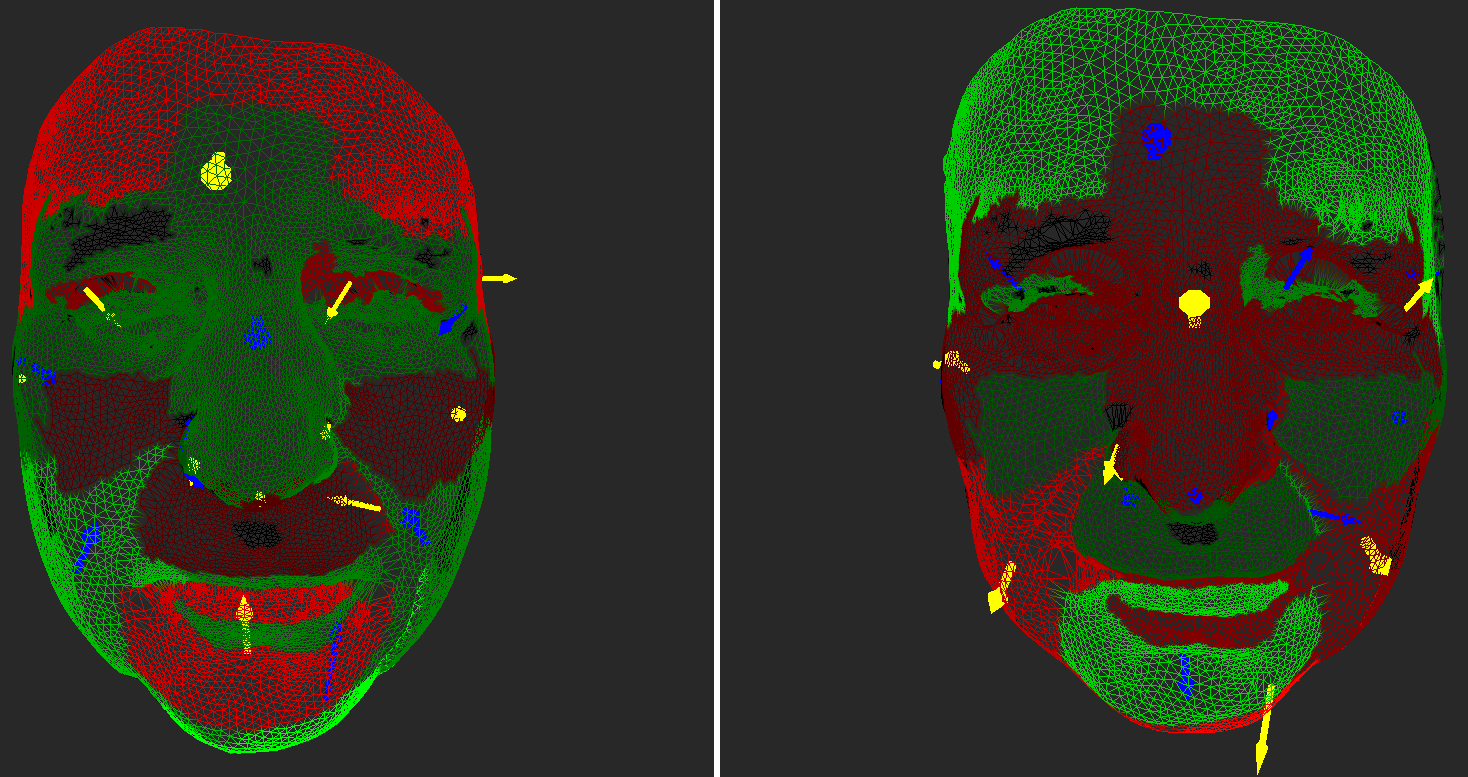
\includegraphics[width=\textwidth]{./screenshots/pair3.PNG}
\caption{}
\label{fig:0-3}
\end{subfigure}
\caption{Visualizations presented to the participants}
\end{figure}
\medskip
\begin{center}
\begin{tabular}{| c | c | c | c | c |}
	\hline
\multirow{2}{*}{\bf Answers} & \ref{fig:0-2} & \ref{fig:0-4} & \ref{fig:0-1} & \ref{fig:0-3}\\
	&  (\(t=20.46\)) &  (\(t=26.19\)) &  (\(t=20.26\)) &  (\(t=21.56\))\\ \hline
	Left & 7 & 8 & 6 & 4\\ \hline
	Right & 4 & 2 & 1 & 2\\ \hline
	NotSure & 2 & 1 & 0 & 0\\ \hline
	{\bf Total} & {\bf 13} & {\bf 11} & {\bf 7} & {\bf 6}\\ \hline
\end{tabular}
\end{center}
\clearpage

\subsection{Question 2}

\begin{center}{\it Does the chin stick out more to the front in the right face than in the left face?}\end{center}

\begin{figure}[h]
\centering
\begin{subfigure}{0.4\textwidth}
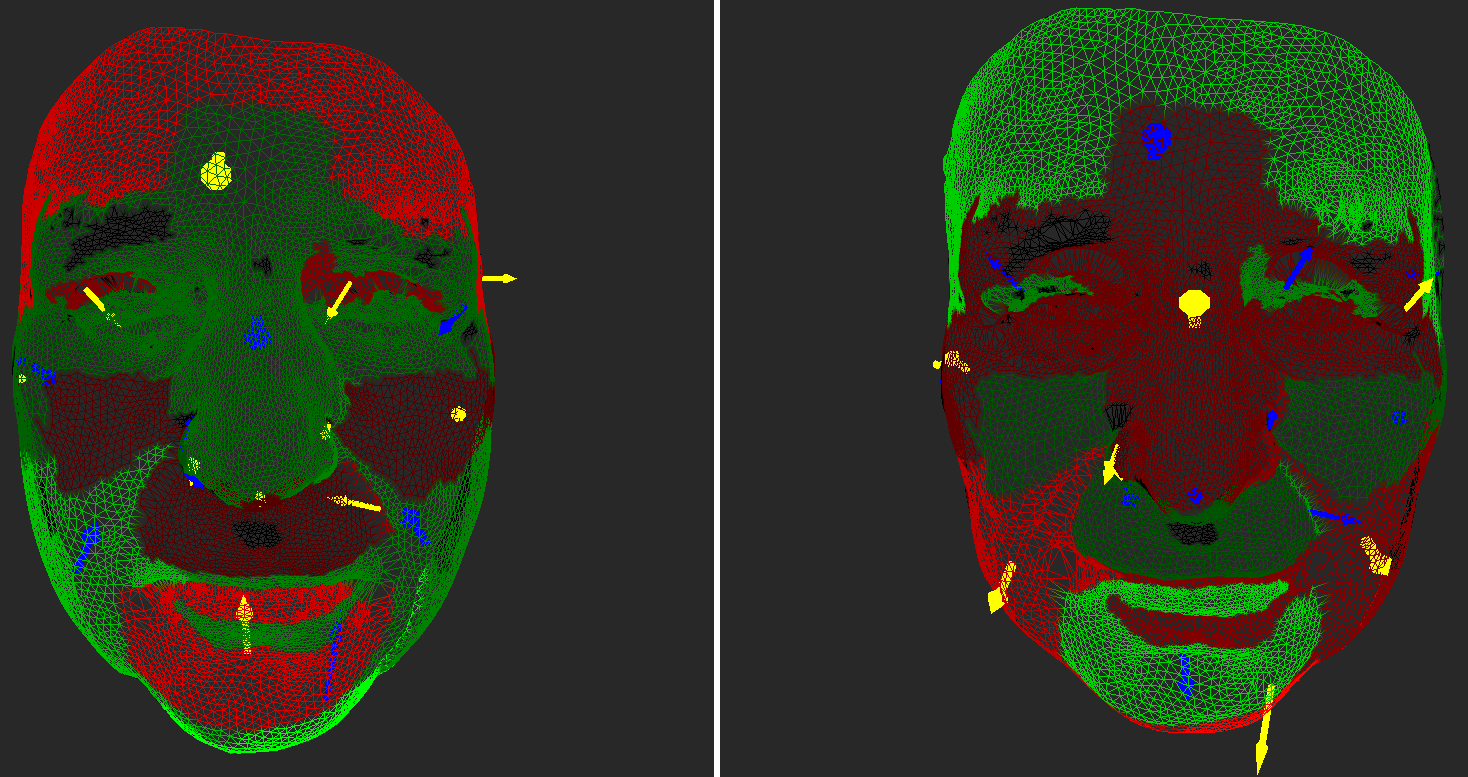
\includegraphics[width=\textwidth]{./screenshots/pair3.PNG}
\caption{}
\label{fig:1-3}
\end{subfigure}
\quad
\begin{subfigure}{0.4\textwidth}
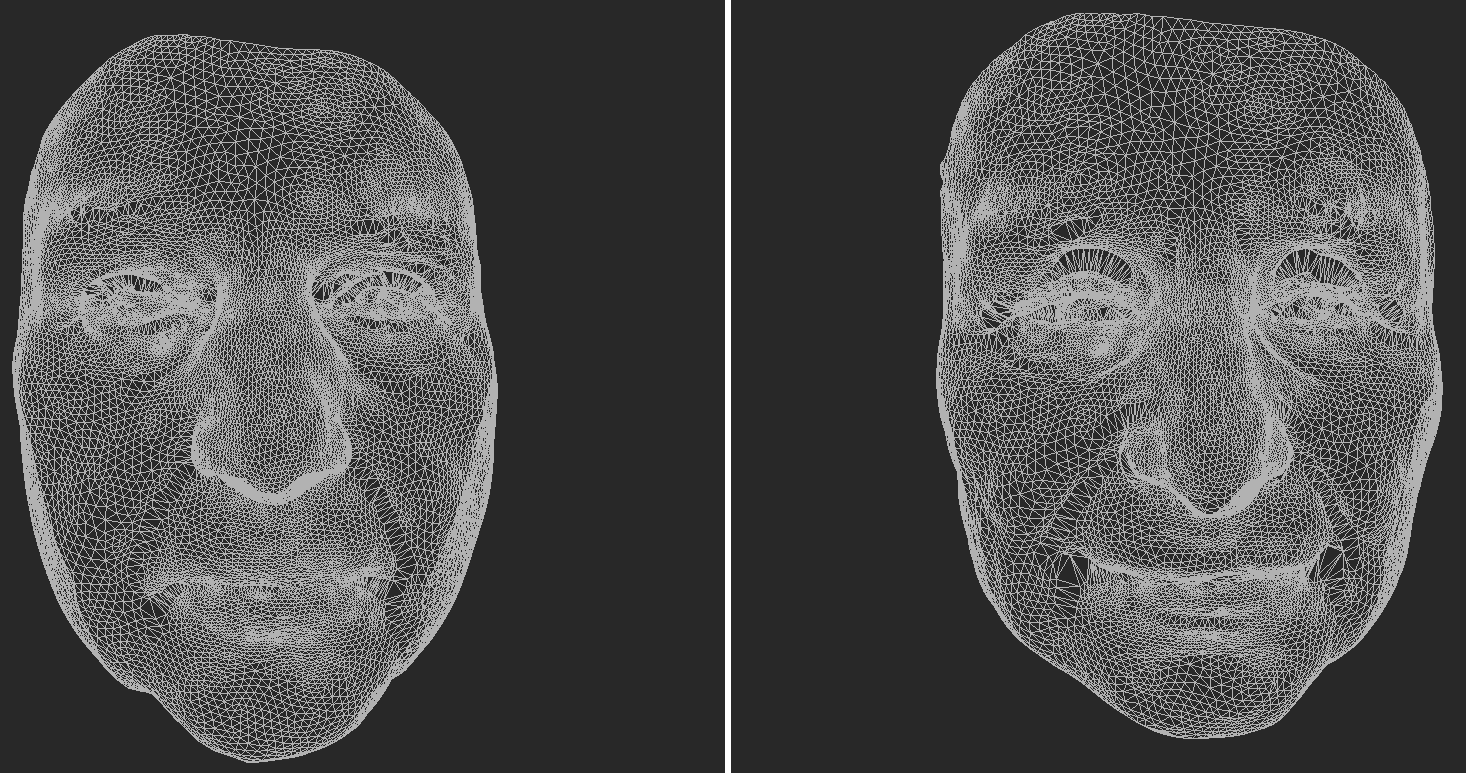
\includegraphics[width=\textwidth]{./screenshots/pair1.PNG}
\caption{}
\label{fig:1-1}
\end{subfigure}

\begin{subfigure}{0.4\textwidth}
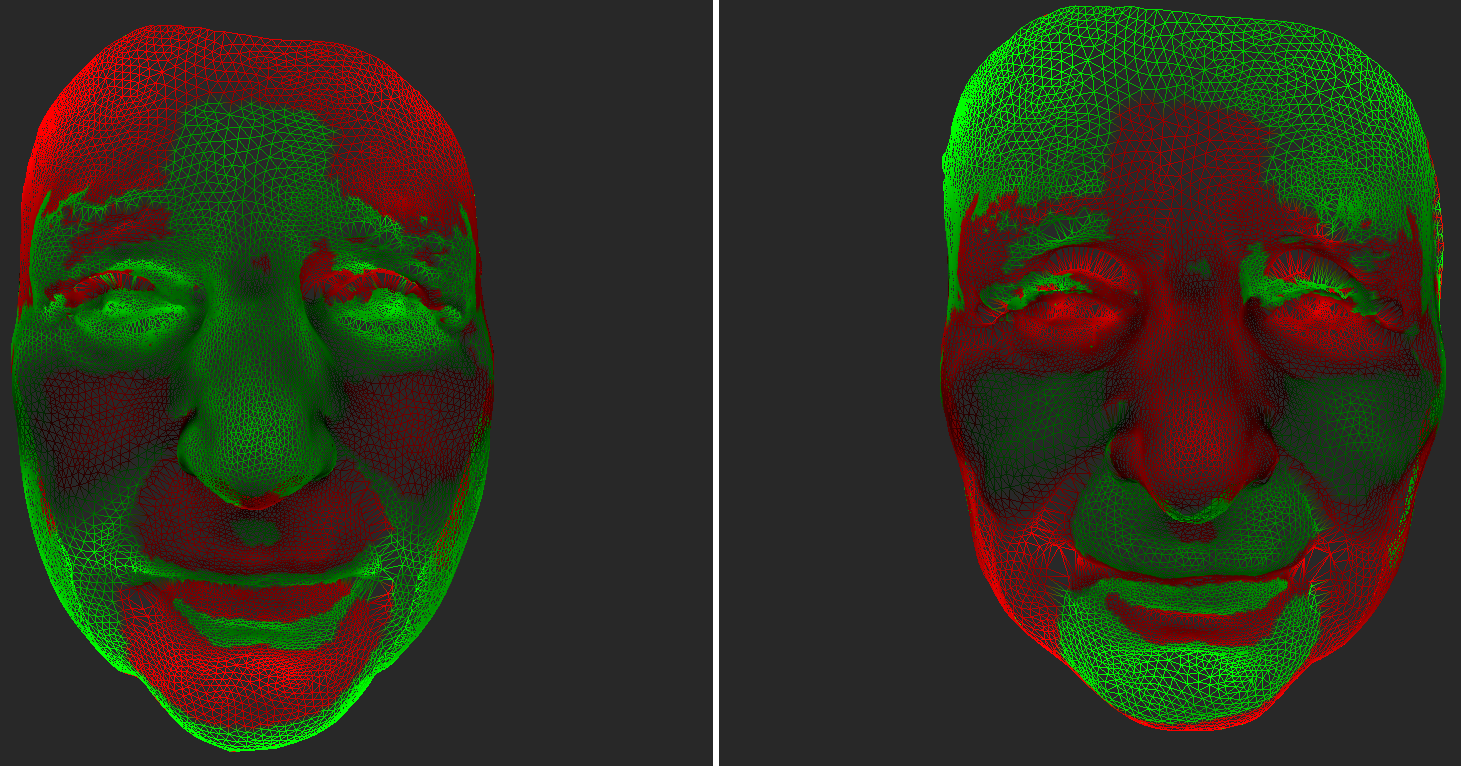
\includegraphics[width=\textwidth]{./screenshots/pair2.PNG}
\caption{}
\label{fig:1-2}
\end{subfigure}
\quad
\begin{subfigure}{0.4\textwidth}
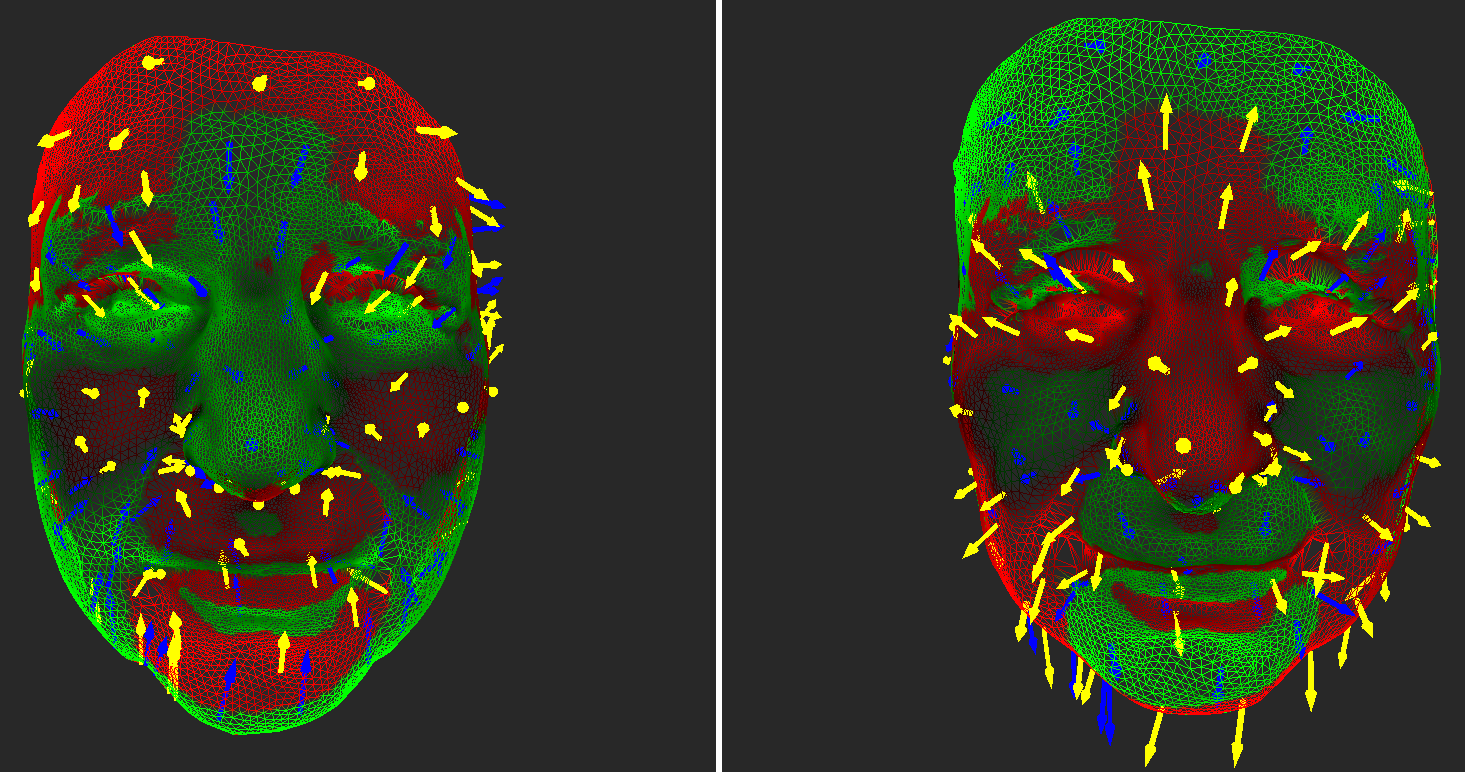
\includegraphics[width=\textwidth]{./screenshots/pair4.PNG}
\caption{}
\label{fig:1-4}
\end{subfigure}
\caption{Visualizations presented to the participants}
\end{figure}
\medskip
\begin{center}
\begin{tabular}{| c | c | c | c | c |}
	\hline
\multirow{2}{*}{\bf Answers} & \ref{fig:1-3} & \ref{fig:1-1} & \ref{fig:1-2} & \ref{fig:1-4}\\
	&  (\(t=46.62\)) &  (\(t=43.08\)) &  (\(t=61.56\)) &  (\(t=38.90\))\\ \hline
	Yes & 10 & 5 & 6 & 4\\ \hline
	No & 3 & 4 & 1 & 2\\ \hline
	NotSure & 0 & 2 & 0 & 0\\ \hline
	{\bf Total} & {\bf 13} & {\bf 11} & {\bf 7} & {\bf 6}\\ \hline
\end{tabular}
\end{center}
\clearpage

\subsection{Question 3}

\begin{center}{\it Where is the most significant difference between the two faces?}\end{center}

\begin{figure}[h]
\centering
\begin{subfigure}{0.4\textwidth}
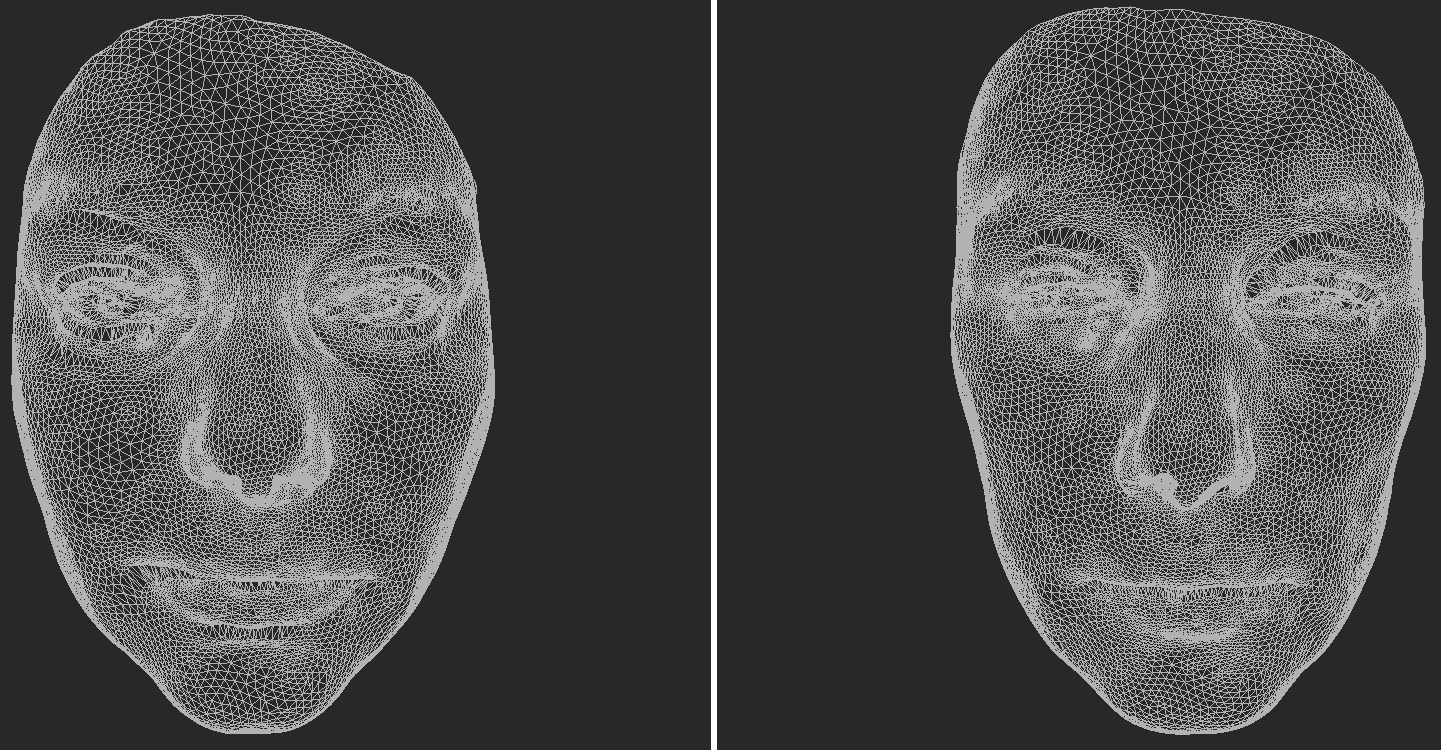
\includegraphics[width=\textwidth]{./screenshots/pair6.PNG}
\caption{}
\label{fig:2-6}
\end{subfigure}
\quad
\begin{subfigure}{0.4\textwidth}
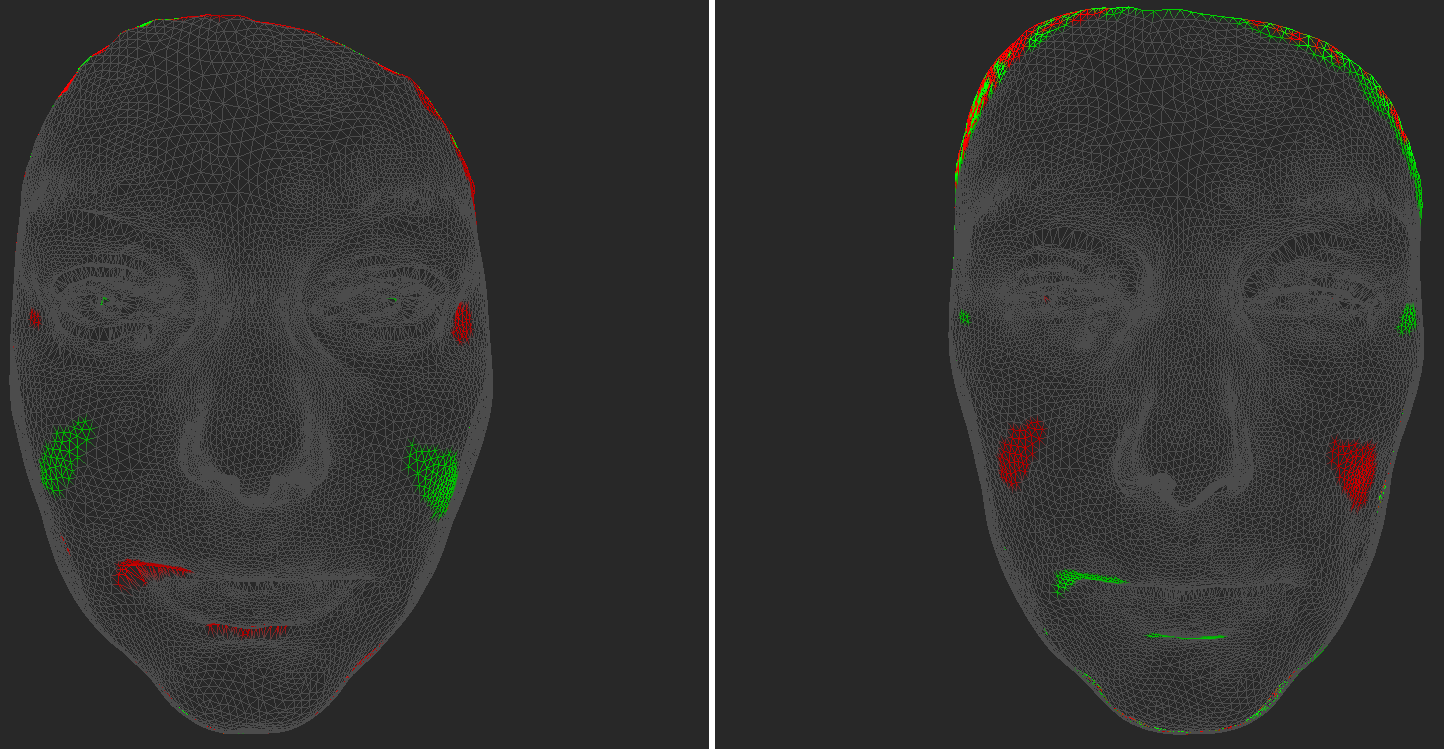
\includegraphics[width=\textwidth]{./screenshots/pair8.PNG}
\caption{}
\label{fig:2-8}
\end{subfigure}

\begin{subfigure}{0.4\textwidth}
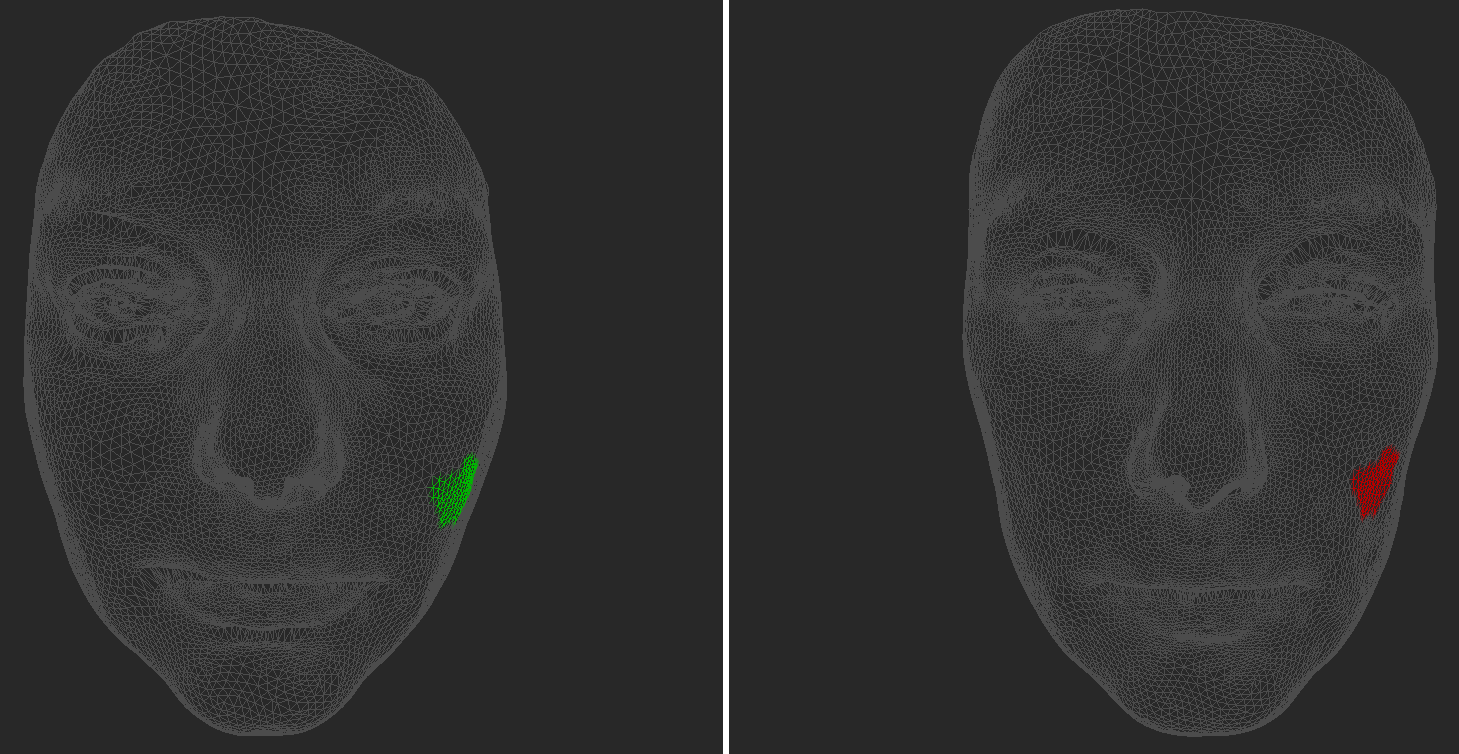
\includegraphics[width=\textwidth]{./screenshots/pair5.PNG}
\caption{}
\label{fig:2-5}
\end{subfigure}
\quad
\begin{subfigure}{0.4\textwidth}
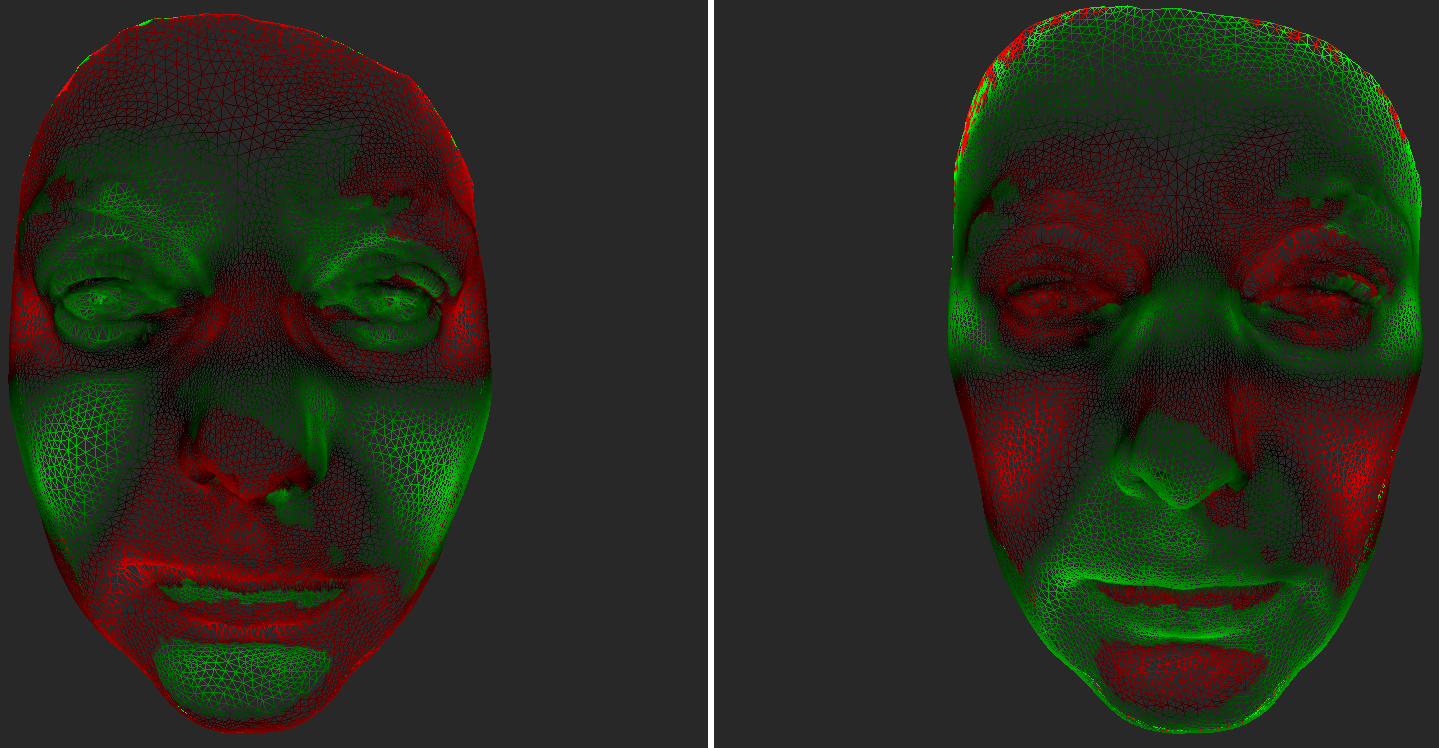
\includegraphics[width=\textwidth]{./screenshots/pair7.PNG}
\caption{}
\label{fig:2-7}
\end{subfigure}
\caption{Visualizations presented to the participants}
\end{figure}
\medskip
\begin{center}
\begin{tabular}{| c | c | c | c | c |}
	\hline
\multirow{2}{*}{\bf Answers} & \ref{fig:2-6} & \ref{fig:2-8} & \ref{fig:2-5} & \ref{fig:2-7}\\
	&  (\(t=41.87\)) &  (\(t=37.36\)) &  (\(t=31.29\)) &  (\(t=58.84\))\\ \hline
	LeftCheek & 2 & 1 & 3 & 1\\ \hline
	Forehead & 5 & 4 & 0 & 1\\ \hline
	RightCheek & 2 & 4 & 2 & 1\\ \hline
	Nose & 1 & 0 & 0 & 0\\ \hline
	NotSure & 2 & 2 & 1 & 1\\ \hline
	Chin & 1 & 0 & 0 & 0\\ \hline
	Mouth & 0 & 0 & 1 & 2\\ \hline
	{\bf Total} & {\bf 13} & {\bf 11} & {\bf 7} & {\bf 6}\\ \hline
\end{tabular}
\end{center}
\clearpage

\subsection{Question 4}

\begin{center}{\it When examining the differences moving from the left face to the right face, what is their main direction in the area below the nose?}\end{center}

\begin{figure}[h]
\centering
\begin{subfigure}{0.4\textwidth}
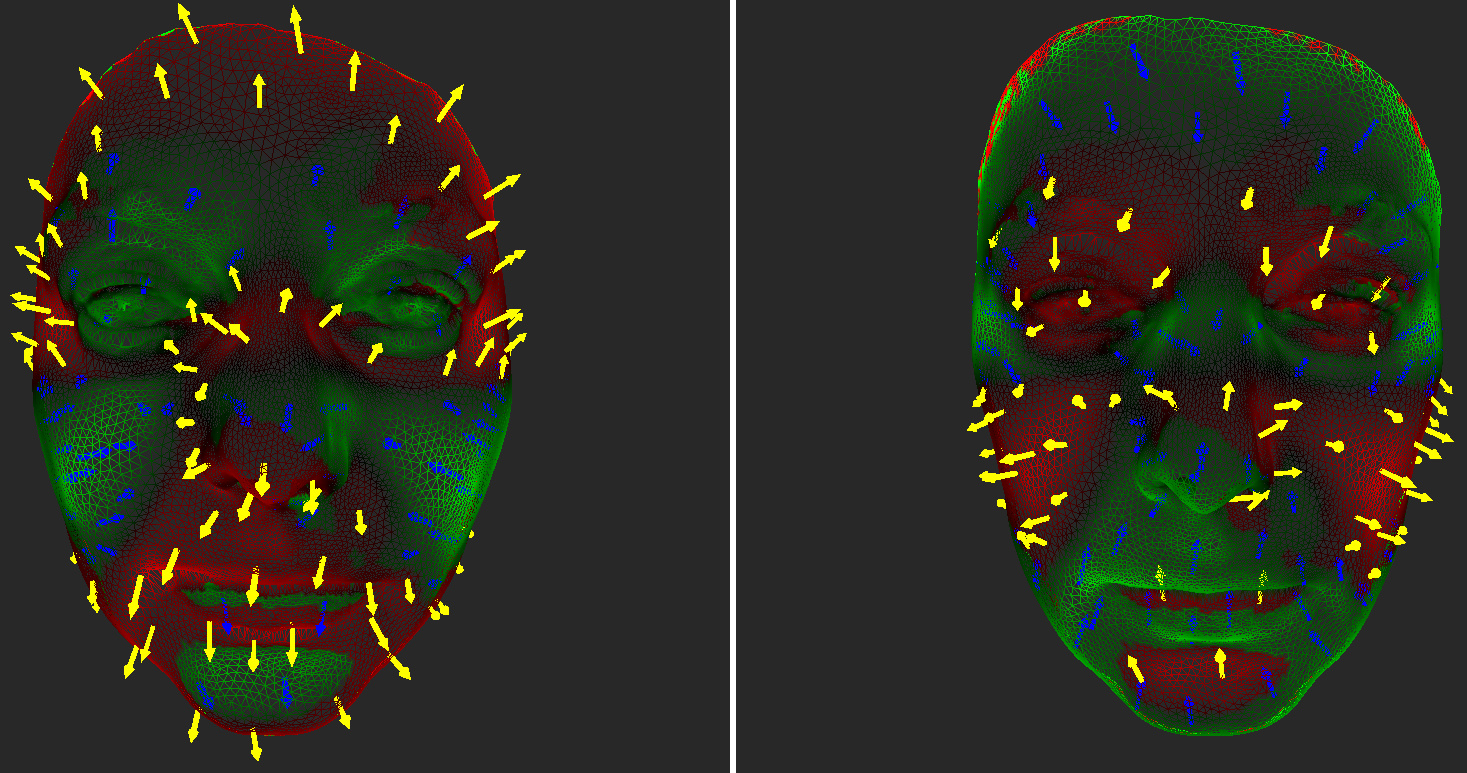
\includegraphics[width=\textwidth]{./screenshots/pair10.PNG}
\caption{}
\label{fig:3-10}
\end{subfigure}
\quad
\begin{subfigure}{0.4\textwidth}
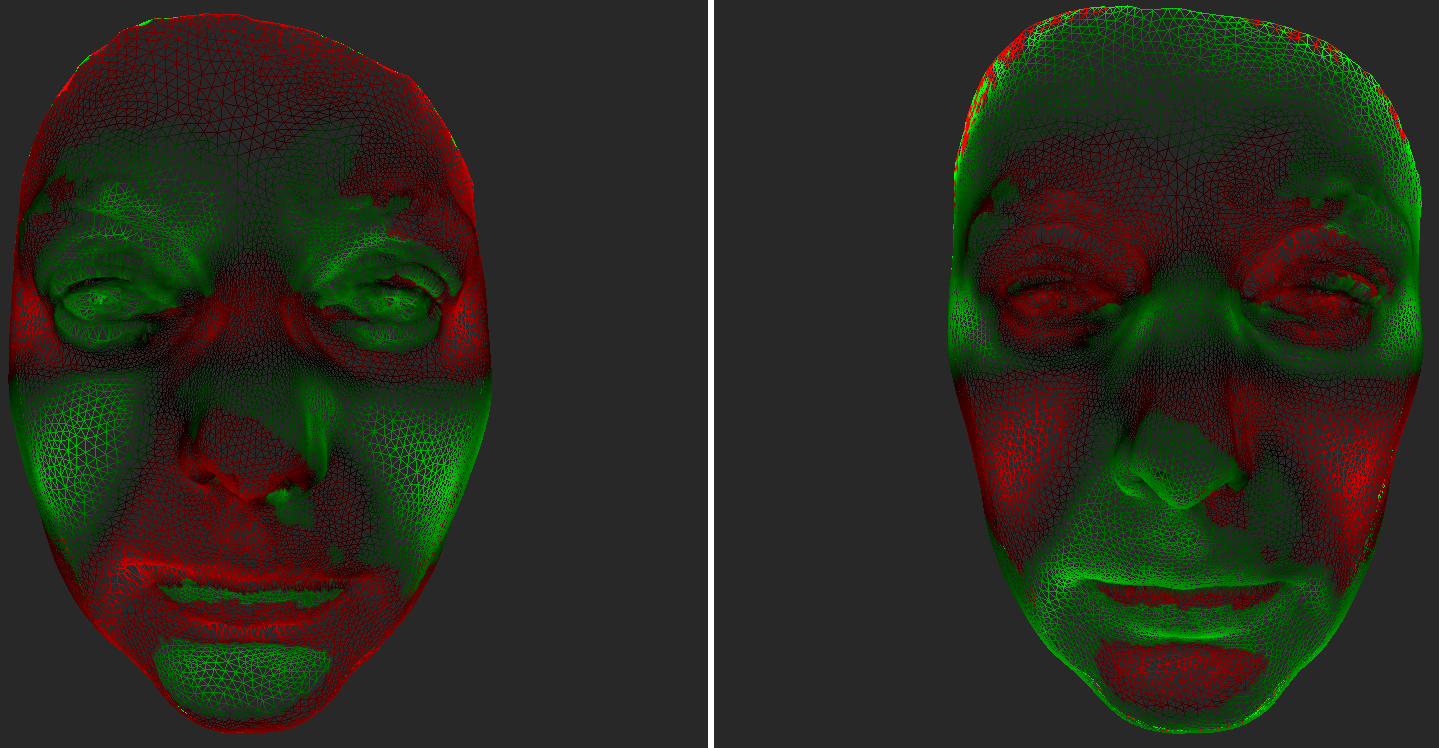
\includegraphics[width=\textwidth]{./screenshots/pair7.PNG}
\caption{}
\label{fig:3-7}
\end{subfigure}

\begin{subfigure}{0.4\textwidth}
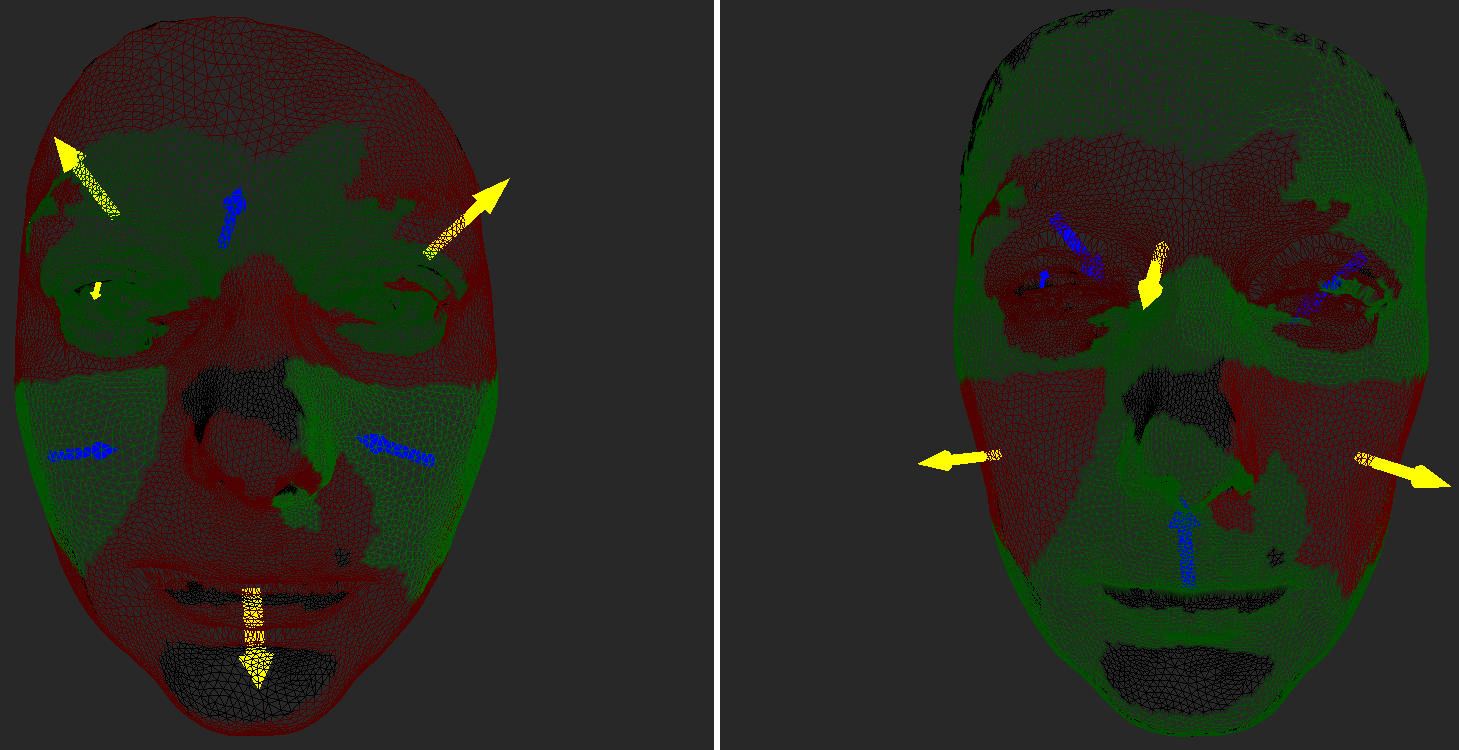
\includegraphics[width=\textwidth]{./screenshots/pair9.PNG}
\caption{}
\label{fig:3-9}
\end{subfigure}
\quad
\begin{subfigure}{0.4\textwidth}
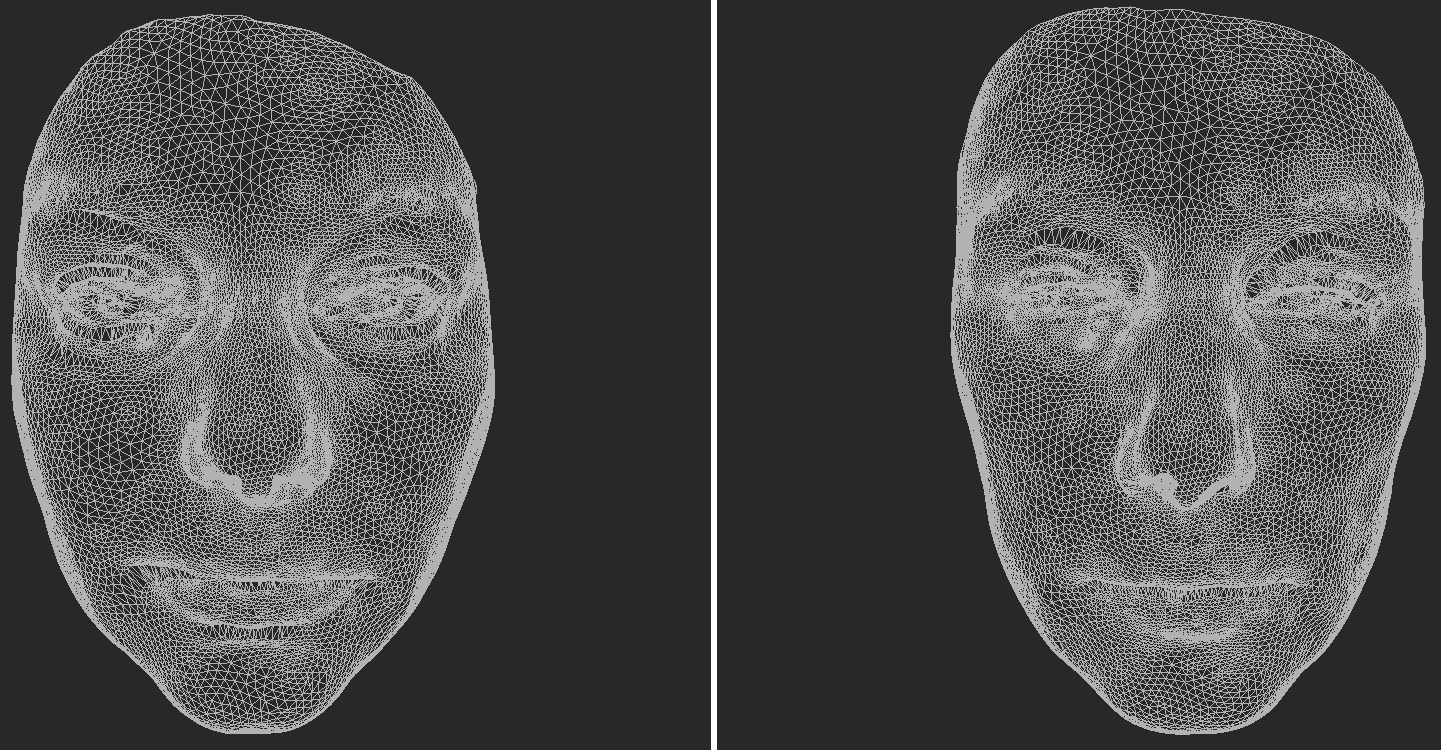
\includegraphics[width=\textwidth]{./screenshots/pair6.PNG}
\caption{}
\label{fig:3-6}
\end{subfigure}
\caption{Visualizations presented to the participants}
\end{figure}
\medskip
\begin{center}
\begin{tabular}{| c | c | c | c | c |}
	\hline
\multirow{2}{*}{\bf Answers} & \ref{fig:3-10} & \ref{fig:3-7} & \ref{fig:3-9} & \ref{fig:3-6}\\
	&  (\(t=48.19\)) &  (\(t=53.41\)) &  (\(t=47.80\)) &  (\(t=55.13\))\\ \hline
	Down & 5 & 2 & 2 & 1\\ \hline
	Right & 1 & 0 & 0 & 1\\ \hline
	In & 2 & 2 & 1 & 0\\ \hline
	NotSure & 2 & 1 & 2 & 2\\ \hline
	Left & 1 & 1 & 0 & 0\\ \hline
	Out & 2 & 5 & 0 & 1\\ \hline
	Up & 0 & 0 & 2 & 1\\ \hline
	{\bf Total} & {\bf 13} & {\bf 11} & {\bf 7} & {\bf 6}\\ \hline
\end{tabular}
\end{center}
\clearpage

\subsection{Question 5}

\begin{center}{\it Does the left cheek stick out more to the front in the right face than in the left face?}\end{center}

\begin{figure}[h]
\centering
\begin{subfigure}{0.4\textwidth}
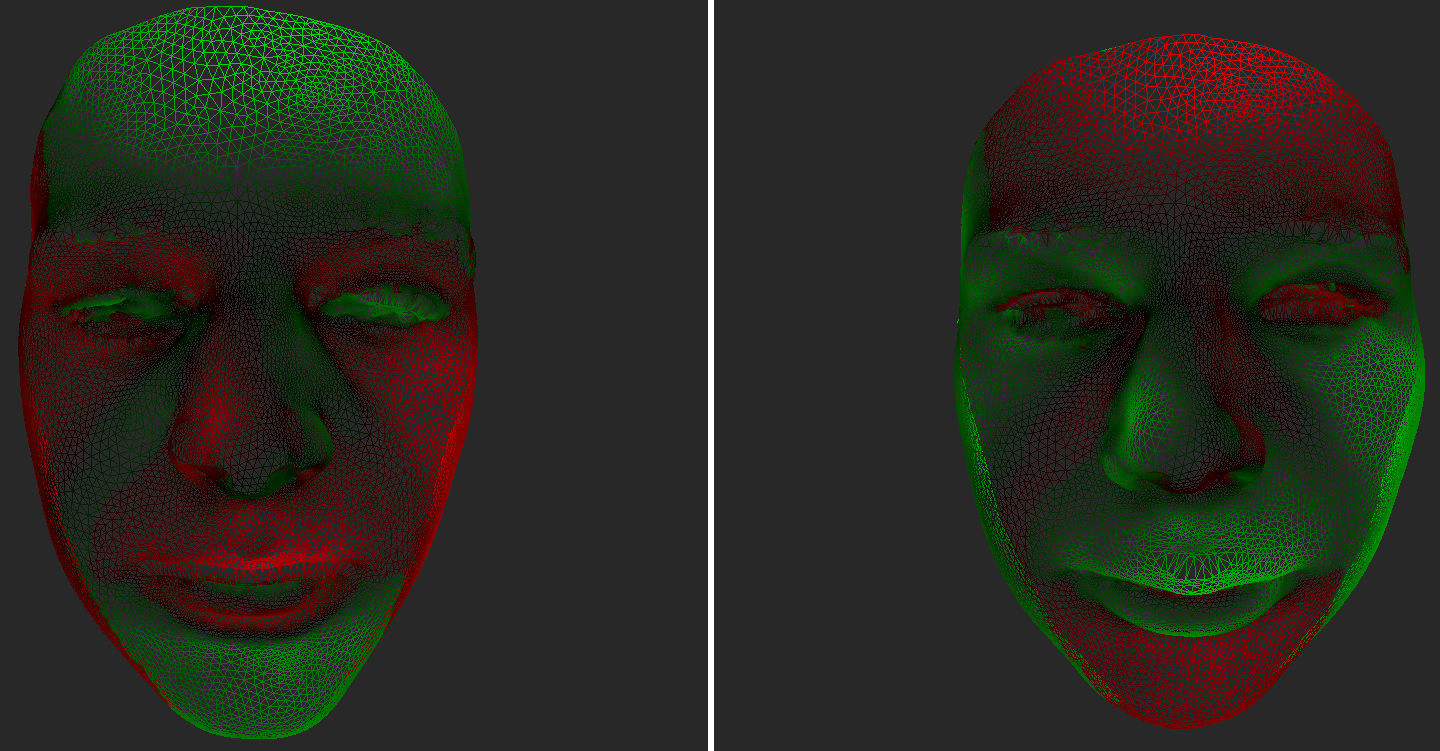
\includegraphics[width=\textwidth]{./screenshots/pair12.PNG}
\caption{}
\label{fig:4-12}
\end{subfigure}
\quad
\begin{subfigure}{0.4\textwidth}
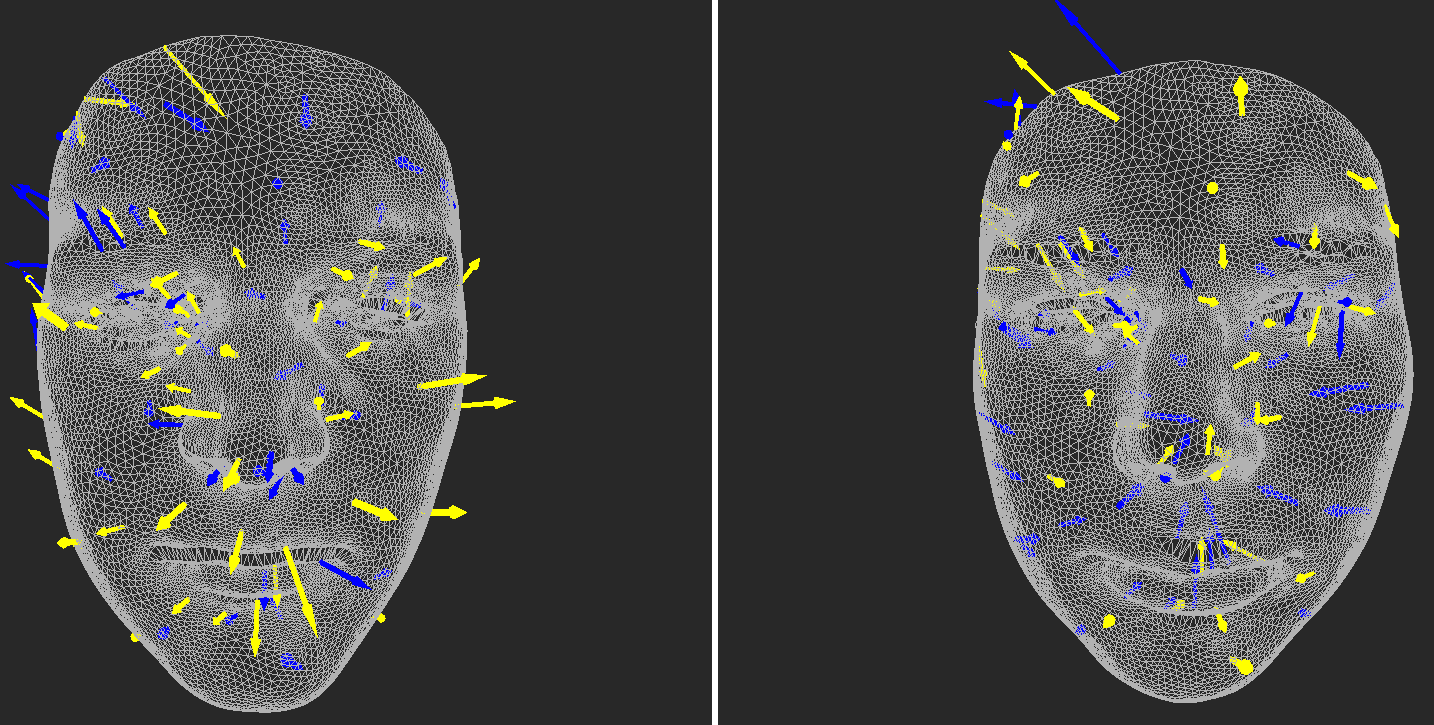
\includegraphics[width=\textwidth]{./screenshots/pair14.PNG}
\caption{}
\label{fig:4-14}
\end{subfigure}

\begin{subfigure}{0.4\textwidth}
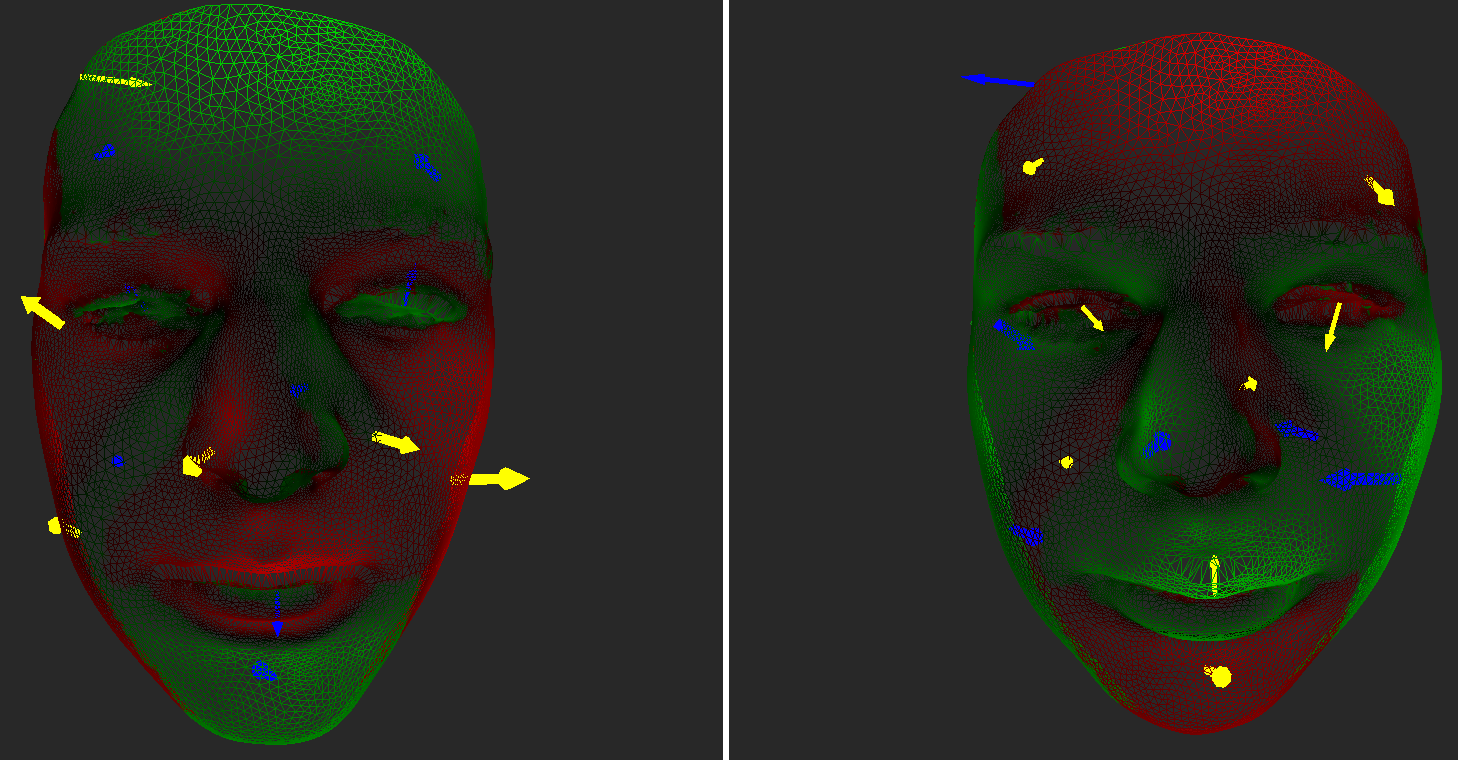
\includegraphics[width=\textwidth]{./screenshots/pair11.PNG}
\caption{}
\label{fig:4-11}
\end{subfigure}
\quad
\begin{subfigure}{0.4\textwidth}
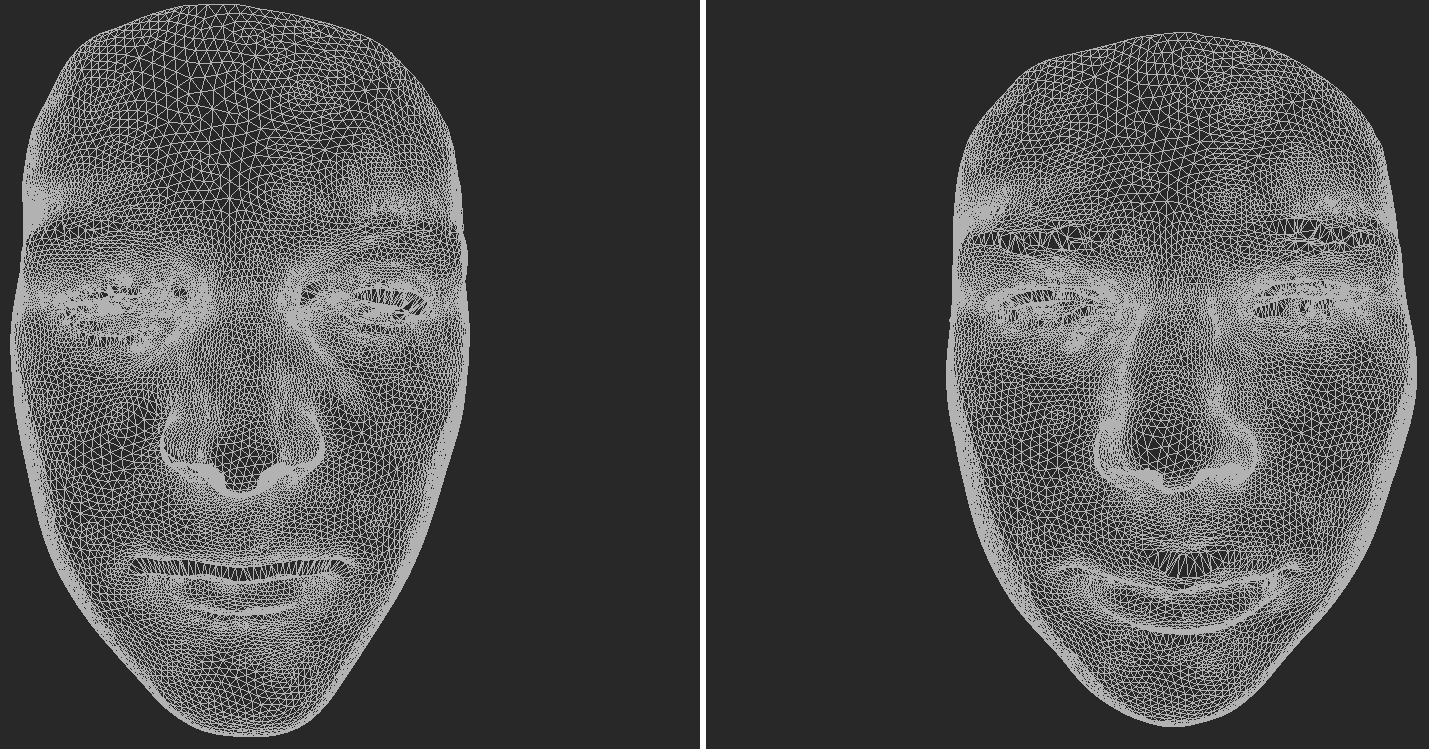
\includegraphics[width=\textwidth]{./screenshots/pair13.PNG}
\caption{}
\label{fig:4-13}
\end{subfigure}
\caption{Visualizations presented to the participants}
\end{figure}
\medskip
\begin{center}
\begin{tabular}{| c | c | c | c | c |}
	\hline
\multirow{2}{*}{\bf Answers} & \ref{fig:4-12} & \ref{fig:4-14} & \ref{fig:4-11} & \ref{fig:4-13}\\
	&  (\(t=40.74\)) &  (\(t=43.85\)) &  (\(t=49.87\)) &  (\(t=31.33\))\\ \hline
	Yes & 8 & 5 & 6 & 3\\ \hline
	No & 5 & 6 & 1 & 3\\ \hline
	{\bf Total} & {\bf 13} & {\bf 11} & {\bf 7} & {\bf 6}\\ \hline
\end{tabular}
\end{center}
\clearpage

\subsection{Question 6}

\begin{center}{\it Which face has a longer nose?}\end{center}

\begin{figure}[h]
\centering
\begin{subfigure}{0.4\textwidth}
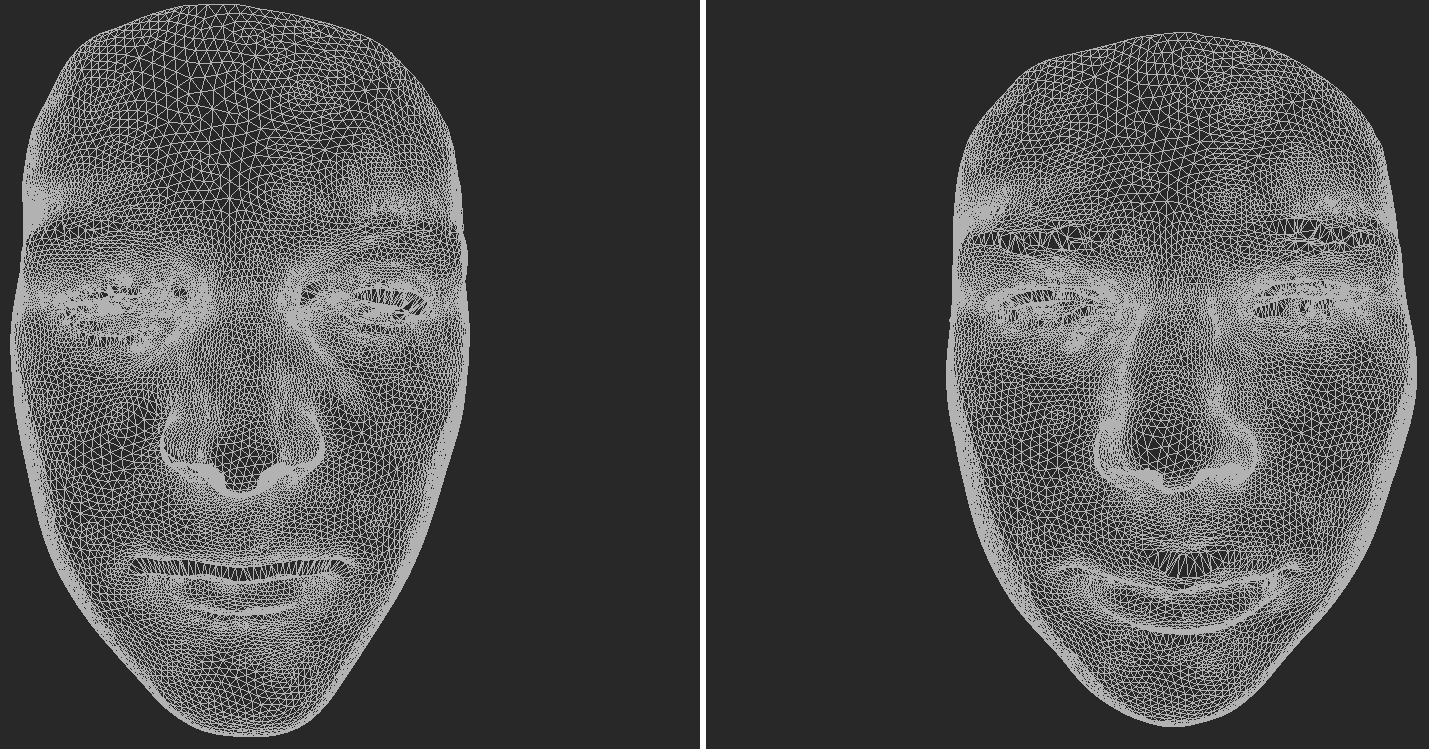
\includegraphics[width=\textwidth]{./screenshots/pair13.PNG}
\caption{}
\label{fig:5-13}
\end{subfigure}
\quad
\begin{subfigure}{0.4\textwidth}
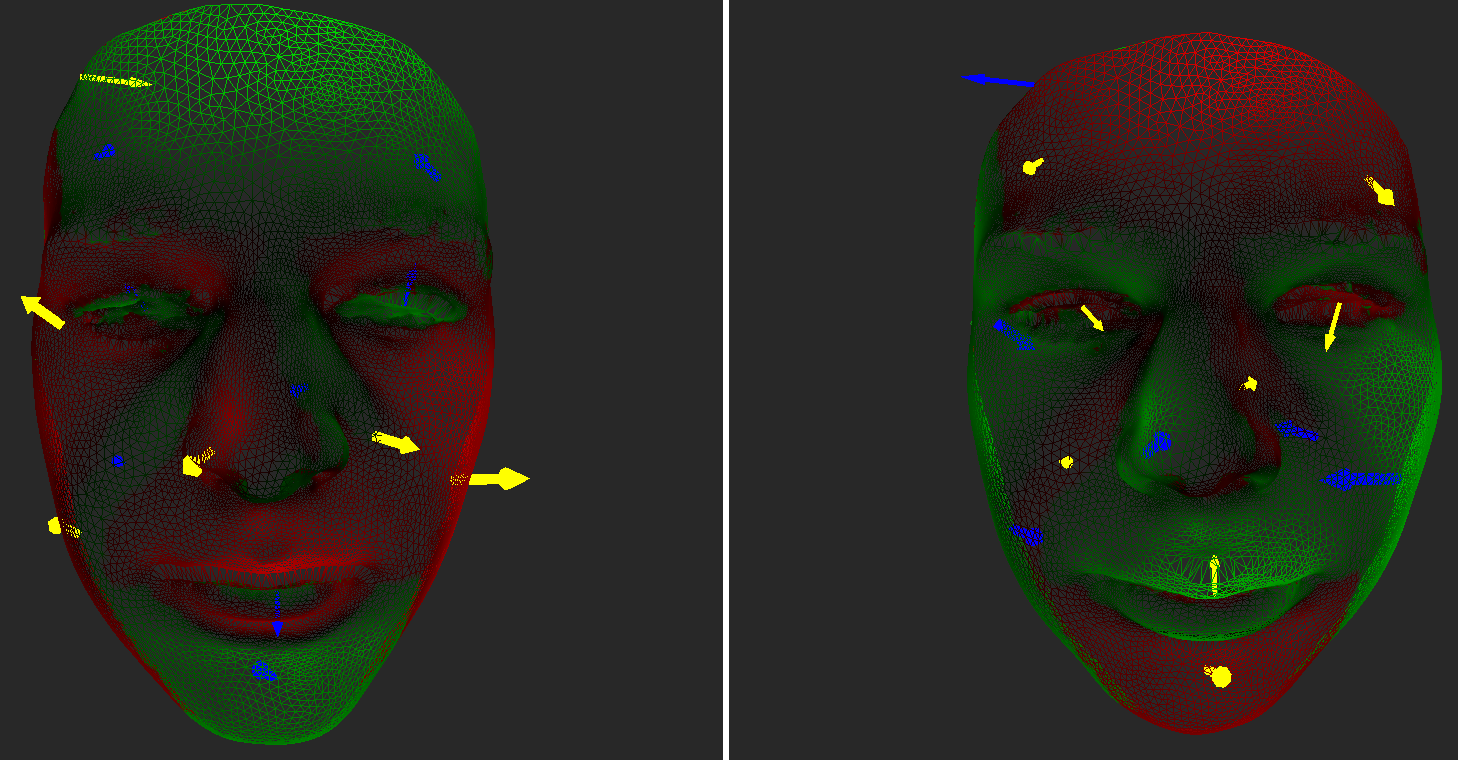
\includegraphics[width=\textwidth]{./screenshots/pair11.PNG}
\caption{}
\label{fig:5-11}
\end{subfigure}

\begin{subfigure}{0.4\textwidth}
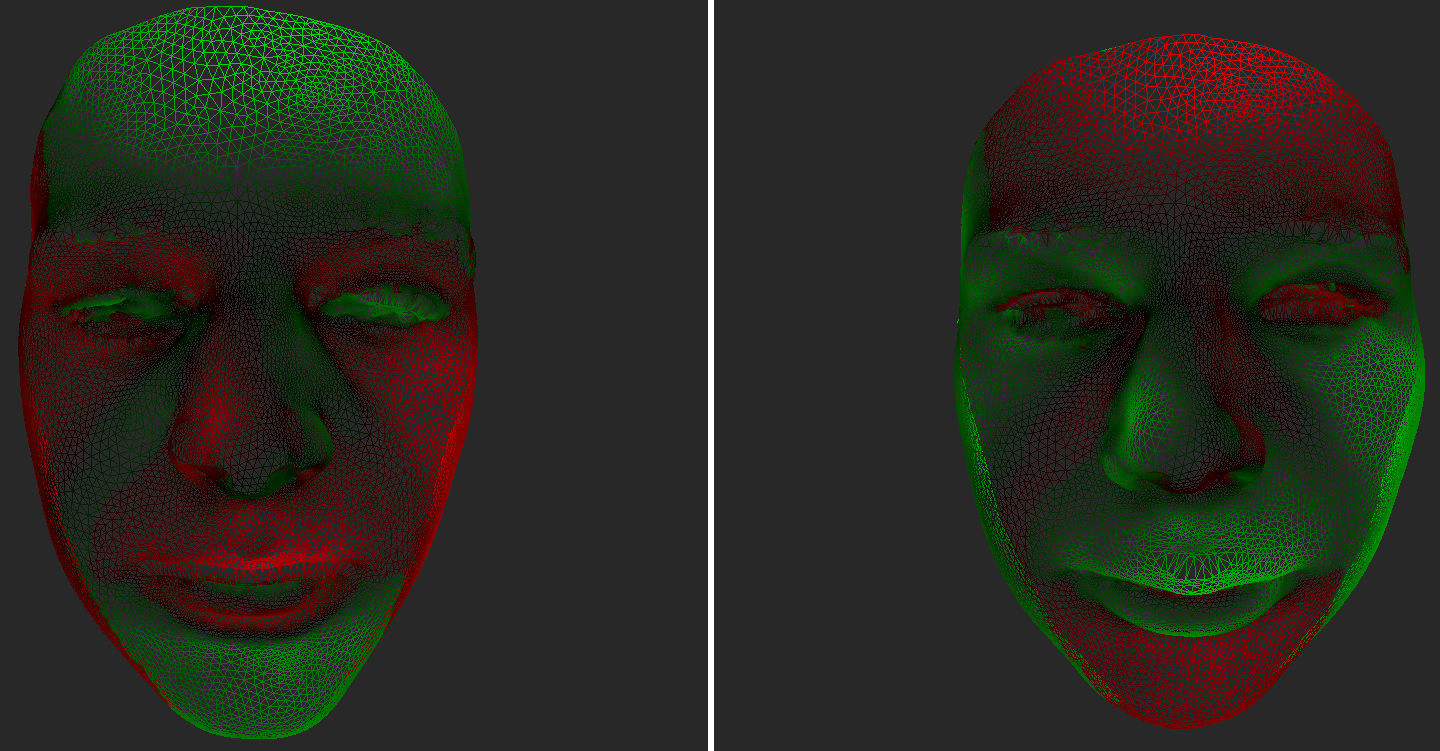
\includegraphics[width=\textwidth]{./screenshots/pair12.PNG}
\caption{}
\label{fig:5-12}
\end{subfigure}
\quad
\begin{subfigure}{0.4\textwidth}
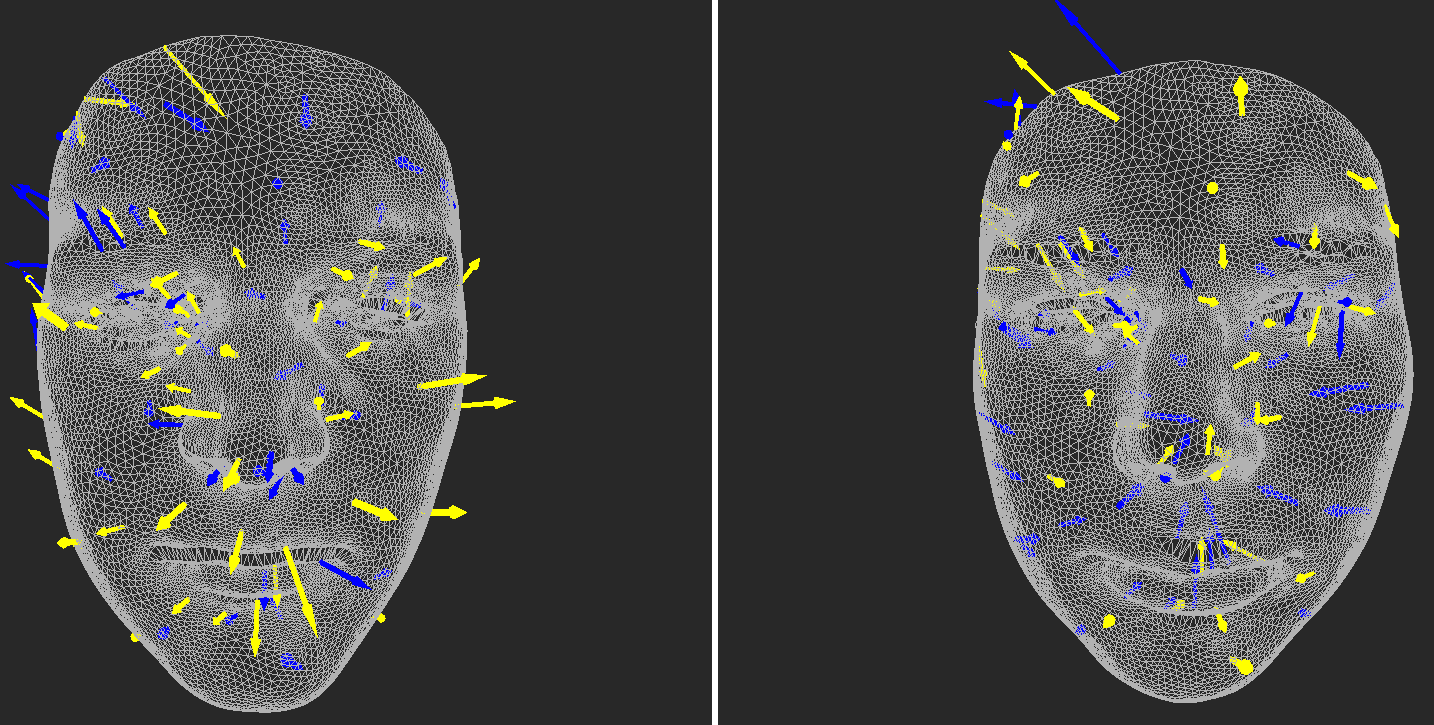
\includegraphics[width=\textwidth]{./screenshots/pair14.PNG}
\caption{}
\label{fig:5-14}
\end{subfigure}
\caption{Visualizations presented to the participants}
\end{figure}
\medskip
\begin{center}
\begin{tabular}{| c | c | c | c | c |}
	\hline
\multirow{2}{*}{\bf Answers} & \ref{fig:5-13} & \ref{fig:5-11} & \ref{fig:5-12} & \ref{fig:5-14}\\
	&  (\(t=33.37\)) &  (\(t=32.34\)) &  (\(t=23.85\)) &  (\(t=29.71\))\\ \hline
	NotSure & 2 & 1 & 0 & 0\\ \hline
	Right & 3 & 5 & 3 & 1\\ \hline
	Left & 8 & 5 & 4 & 5\\ \hline
	{\bf Total} & {\bf 13} & {\bf 11} & {\bf 7} & {\bf 6}\\ \hline
\end{tabular}
\end{center}
\clearpage

\subsection{Question 7}

\begin{center}{\it Which face has larger cheekbones?}\end{center}

\begin{figure}[h]
\centering
\begin{subfigure}{0.4\textwidth}
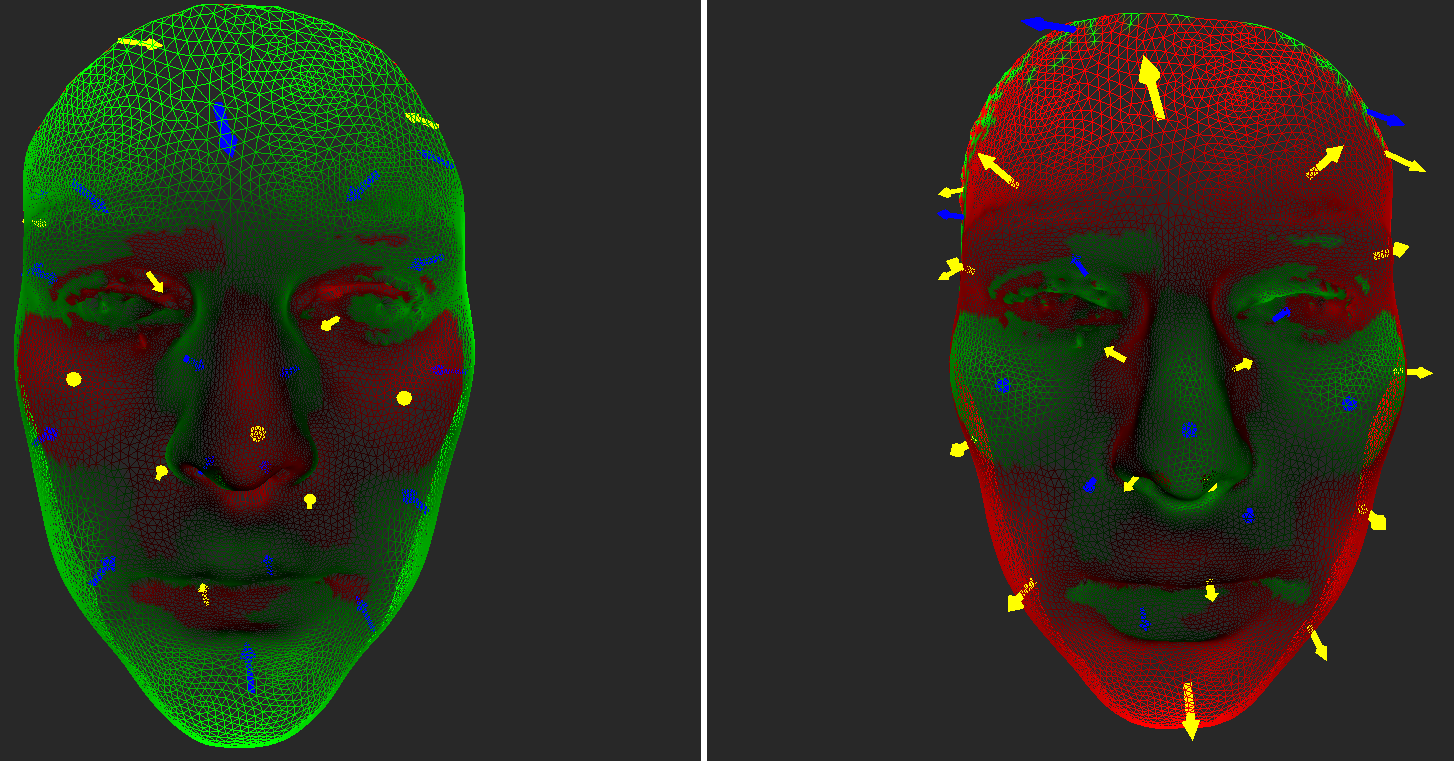
\includegraphics[width=\textwidth]{./screenshots/pair17.PNG}
\caption{}
\label{fig:6-17}
\end{subfigure}
\quad
\begin{subfigure}{0.4\textwidth}
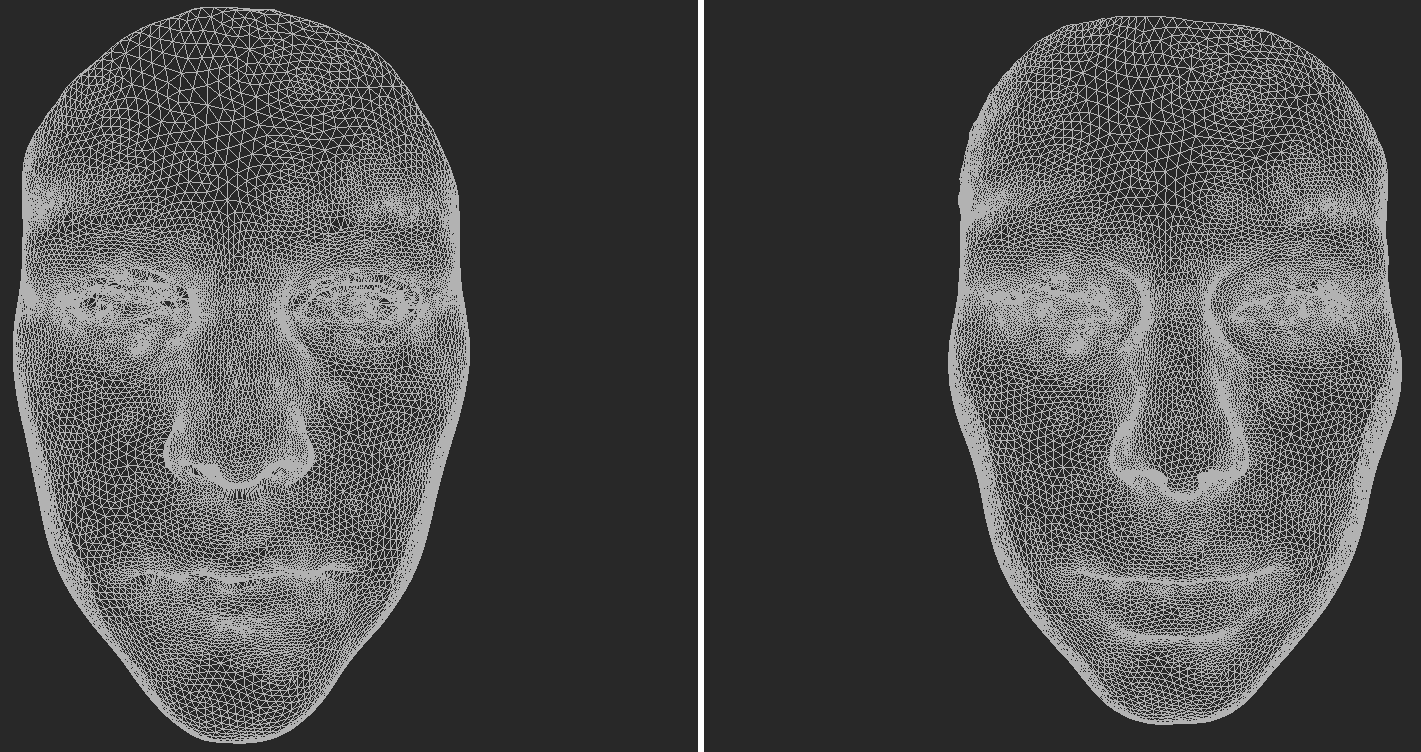
\includegraphics[width=\textwidth]{./screenshots/pair15.PNG}
\caption{}
\label{fig:6-15}
\end{subfigure}

\begin{subfigure}{0.4\textwidth}
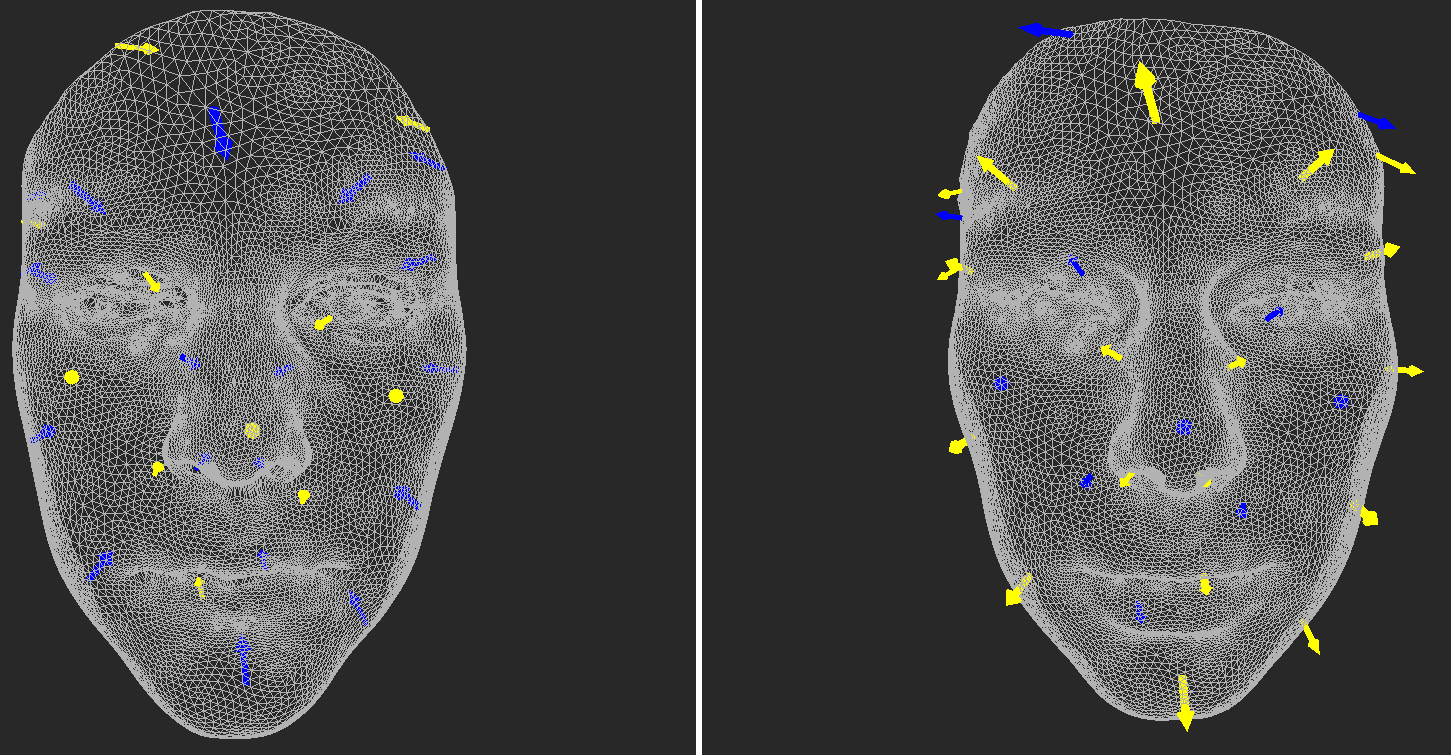
\includegraphics[width=\textwidth]{./screenshots/pair18.PNG}
\caption{}
\label{fig:6-18}
\end{subfigure}
\quad
\begin{subfigure}{0.4\textwidth}
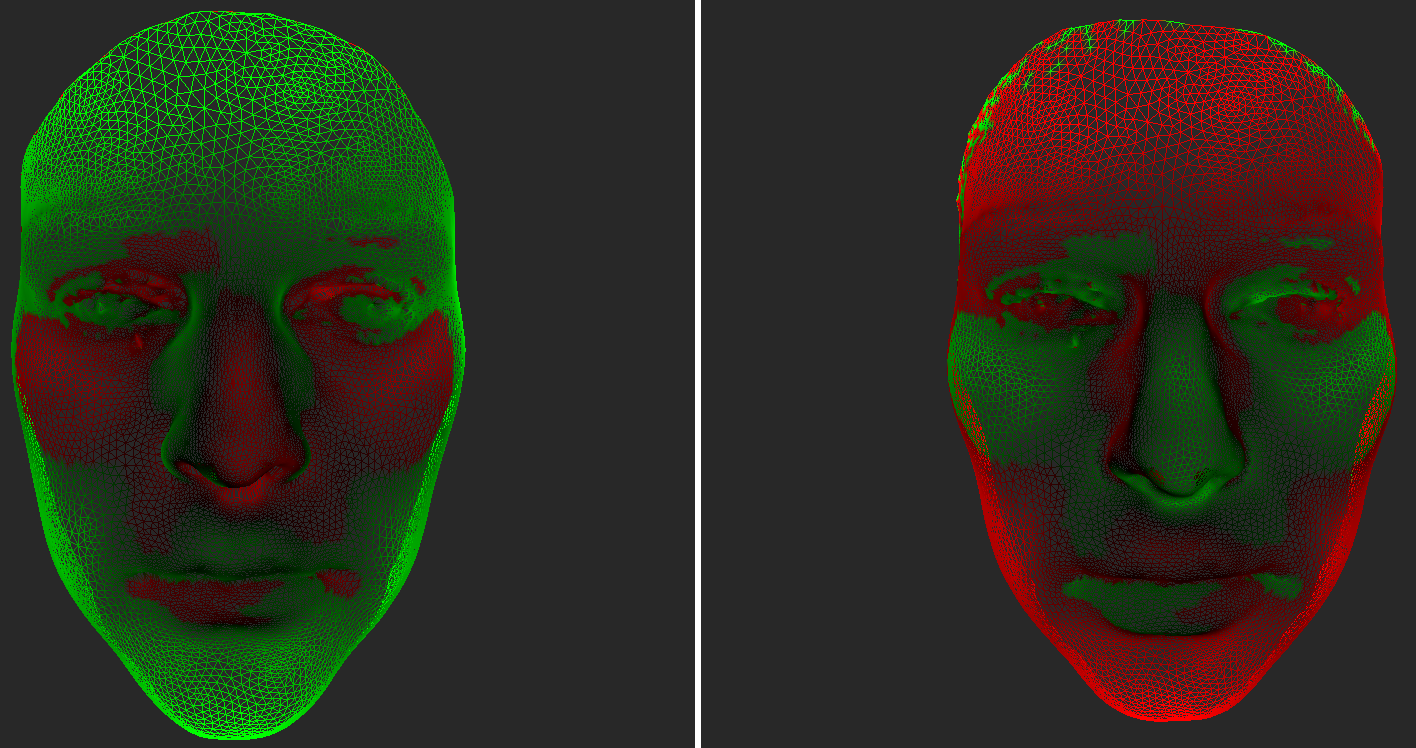
\includegraphics[width=\textwidth]{./screenshots/pair16.PNG}
\caption{}
\label{fig:6-16}
\end{subfigure}
\caption{Visualizations presented to the participants}
\end{figure}
\medskip
\begin{center}
\begin{tabular}{| c | c | c | c | c |}
	\hline
\multirow{2}{*}{\bf Answers} & \ref{fig:6-17} & \ref{fig:6-15} & \ref{fig:6-18} & \ref{fig:6-16}\\
	&  (\(t=16.11\)) &  (\(t=24.59\)) &  (\(t=18.47\)) &  (\(t=15.01\))\\ \hline
	Right & 11 & 4 & 6 & 5\\ \hline
	Left & 2 & 4 & 0 & 1\\ \hline
	NotSure & 0 & 3 & 1 & 0\\ \hline
	{\bf Total} & {\bf 13} & {\bf 11} & {\bf 7} & {\bf 6}\\ \hline
\end{tabular}
\end{center}
\clearpage

\subsection{Question 8}

\begin{center}{\it Which face has a larger eyebrow bone?}\end{center}

\begin{figure}[h]
\centering
\begin{subfigure}{0.4\textwidth}
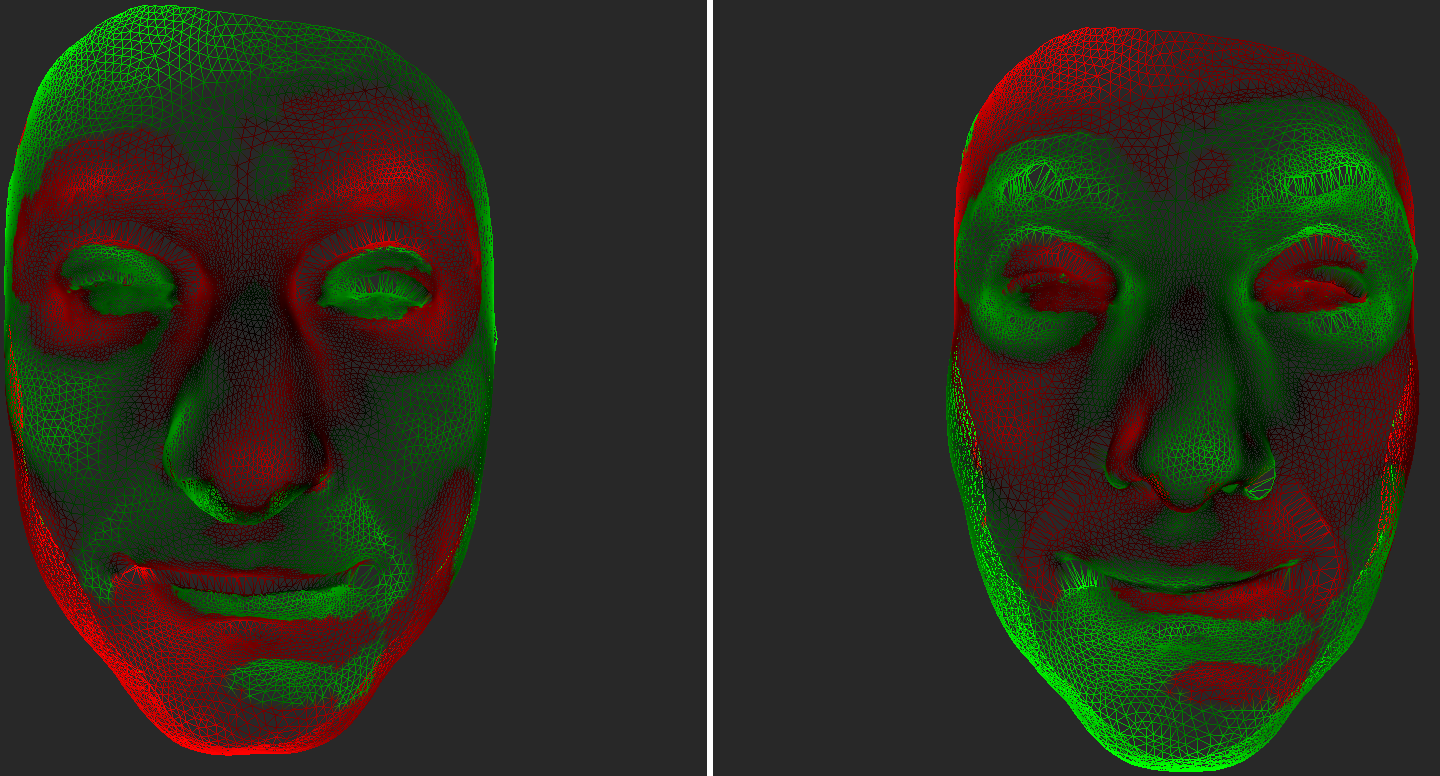
\includegraphics[width=\textwidth]{./screenshots/pair20.PNG}
\caption{}
\label{fig:7-20}
\end{subfigure}
\quad
\begin{subfigure}{0.4\textwidth}
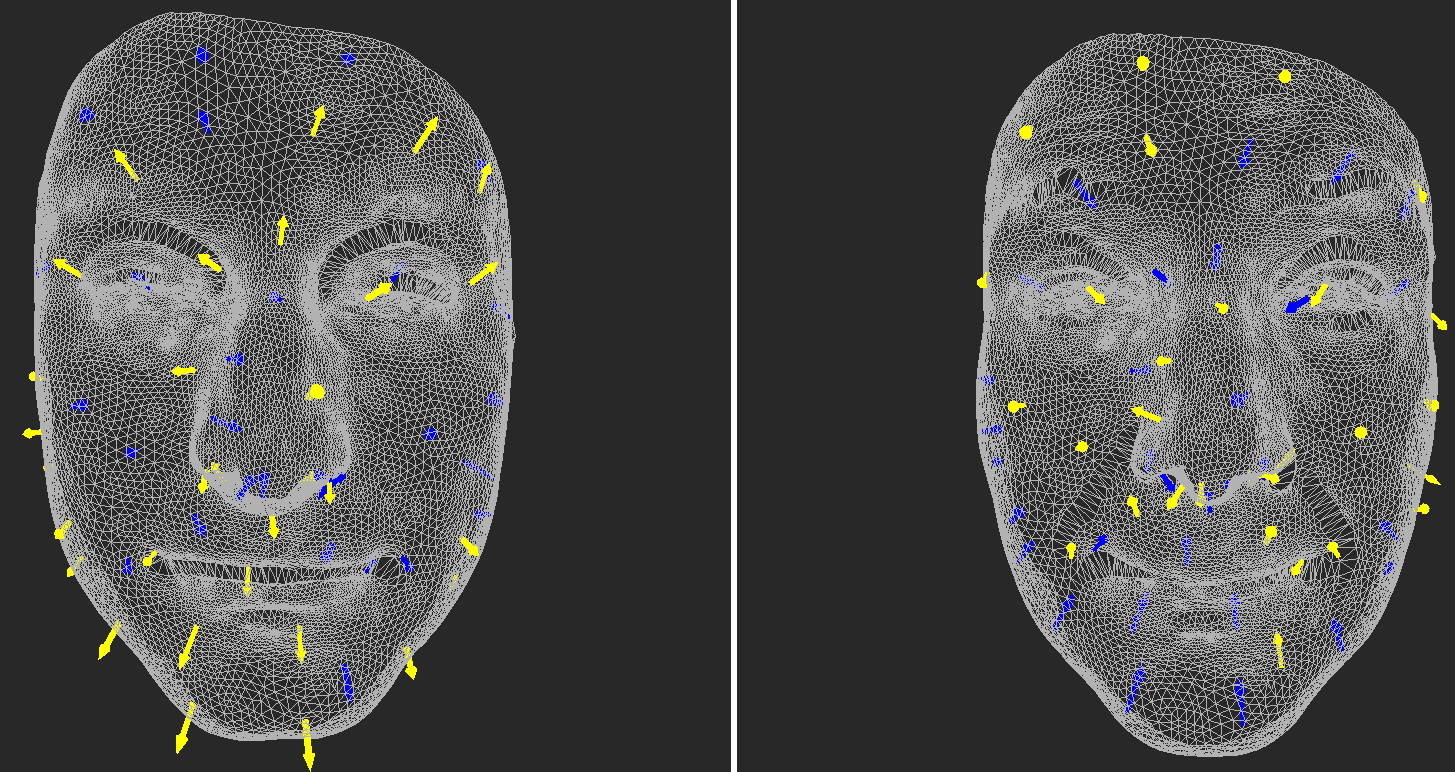
\includegraphics[width=\textwidth]{./screenshots/pair22.PNG}
\caption{}
\label{fig:7-22}
\end{subfigure}

\begin{subfigure}{0.4\textwidth}
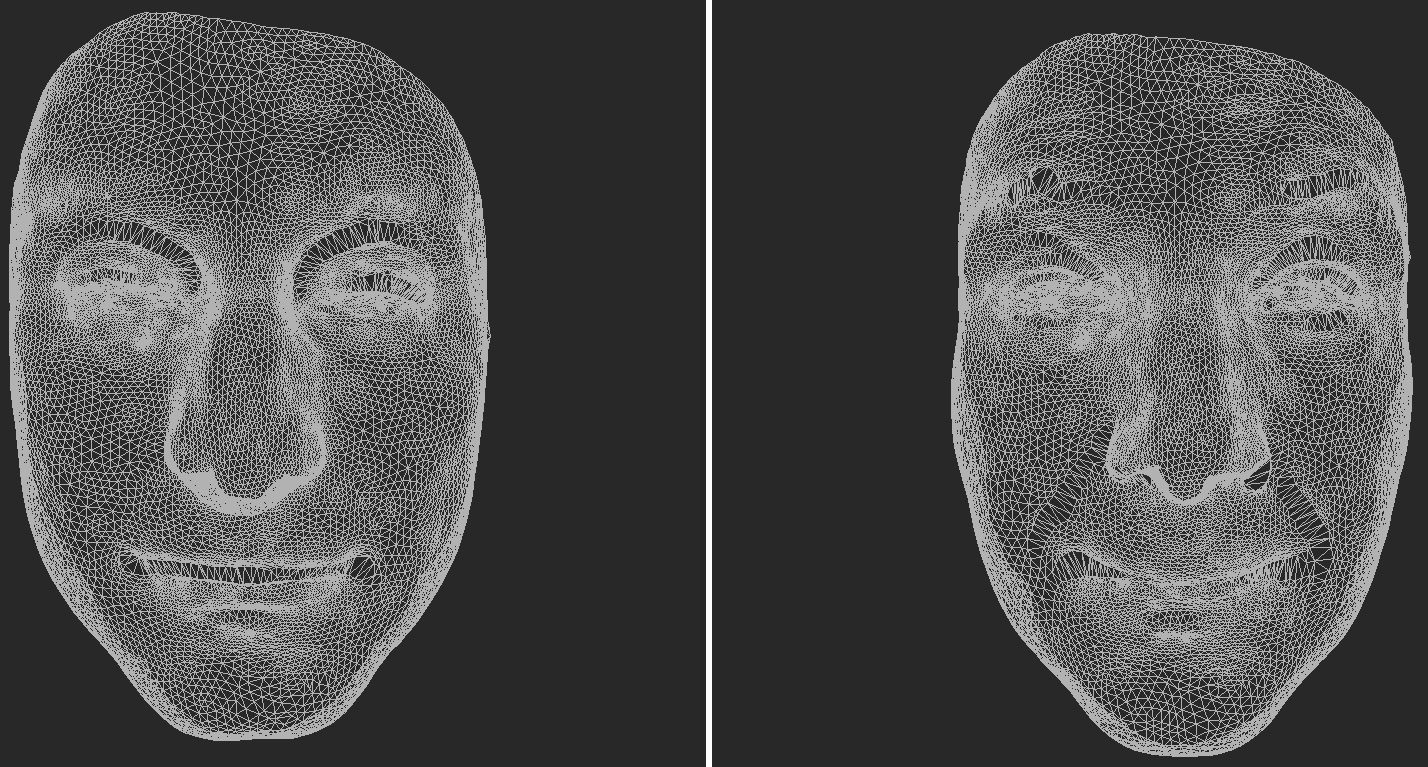
\includegraphics[width=\textwidth]{./screenshots/pair19.PNG}
\caption{}
\label{fig:7-19}
\end{subfigure}
\quad
\begin{subfigure}{0.4\textwidth}
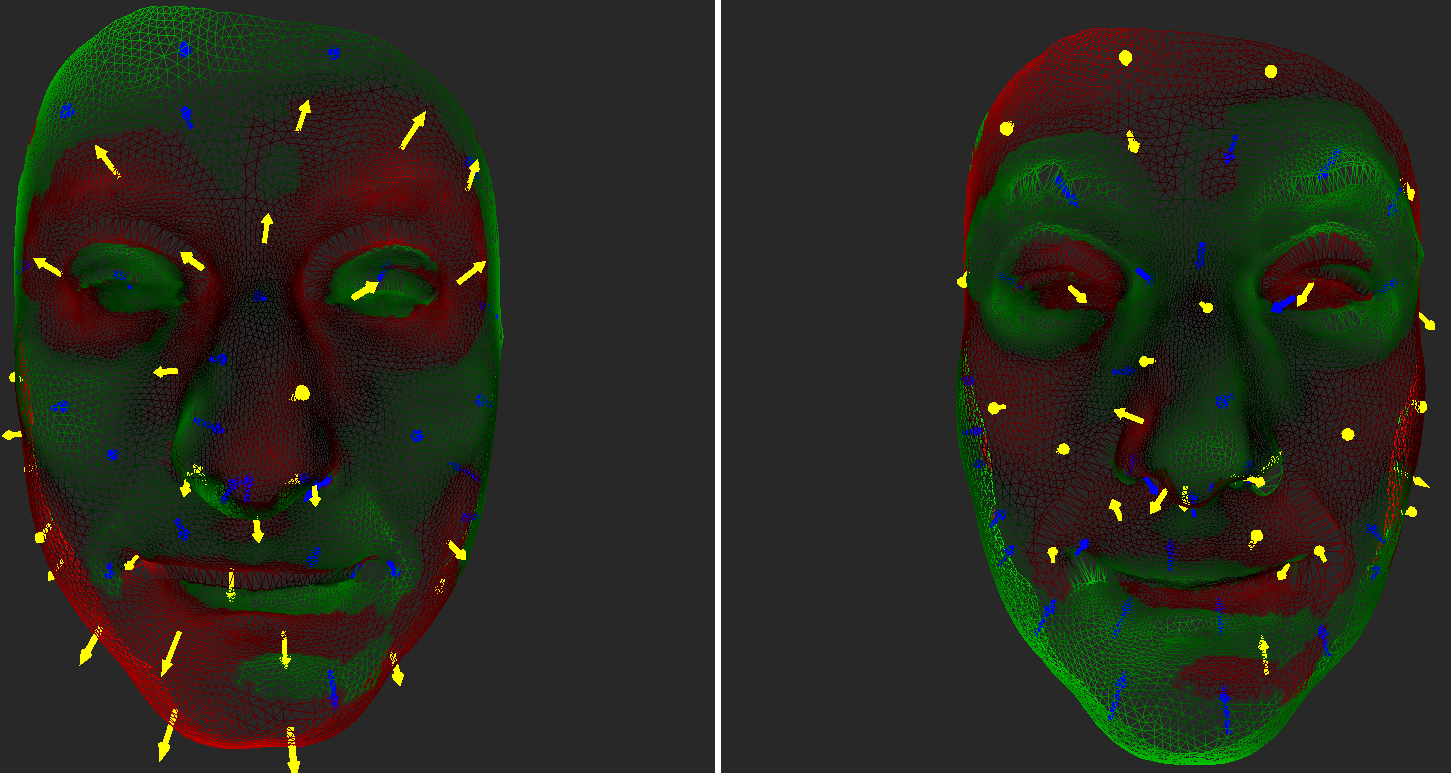
\includegraphics[width=\textwidth]{./screenshots/pair21.PNG}
\caption{}
\label{fig:7-21}
\end{subfigure}
\caption{Visualizations presented to the participants}
\end{figure}
\medskip
\begin{center}
\begin{tabular}{| c | c | c | c | c |}
	\hline
\multirow{2}{*}{\bf Answers} & \ref{fig:7-20} & \ref{fig:7-22} & \ref{fig:7-19} & \ref{fig:7-21}\\
	&  (\(t=17.00\)) &  (\(t=16.25\)) &  (\(t=24.09\)) &  (\(t=16.03\))\\ \hline
	Right & 12 & 8 & 4 & 5\\ \hline
	NotSure & 1 & 0 & 0 & 0\\ \hline
	Left & 0 & 3 & 3 & 1\\ \hline
	{\bf Total} & {\bf 13} & {\bf 11} & {\bf 7} & {\bf 6}\\ \hline
\end{tabular}
\end{center}
\clearpage

\subsection{Question 9}

\begin{center}{\it Where are the two faces the most similar?}\end{center}

\begin{figure}[h]
\centering
\begin{subfigure}{0.4\textwidth}
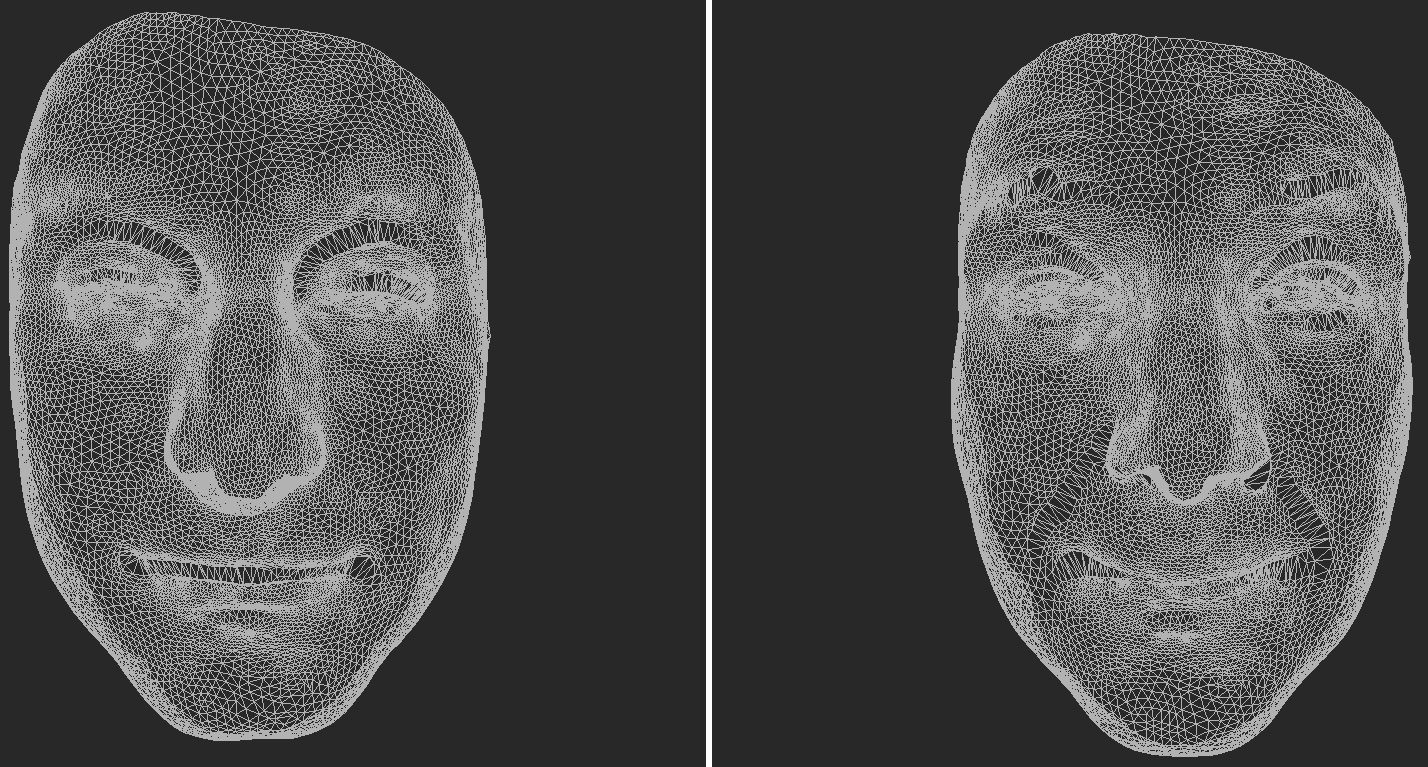
\includegraphics[width=\textwidth]{./screenshots/pair19.PNG}
\caption{}
\label{fig:8-19}
\end{subfigure}
\quad
\begin{subfigure}{0.4\textwidth}
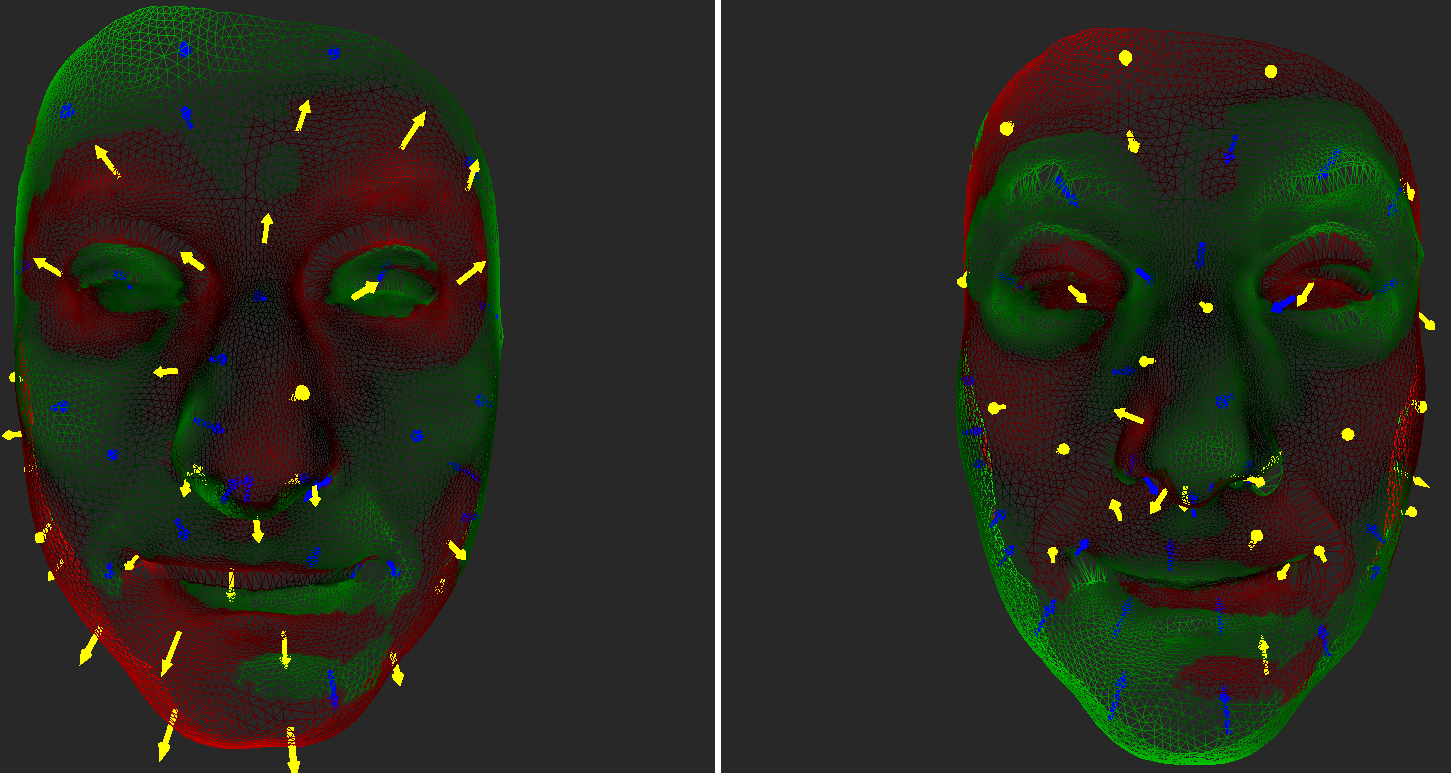
\includegraphics[width=\textwidth]{./screenshots/pair21.PNG}
\caption{}
\label{fig:8-21}
\end{subfigure}

\begin{subfigure}{0.4\textwidth}
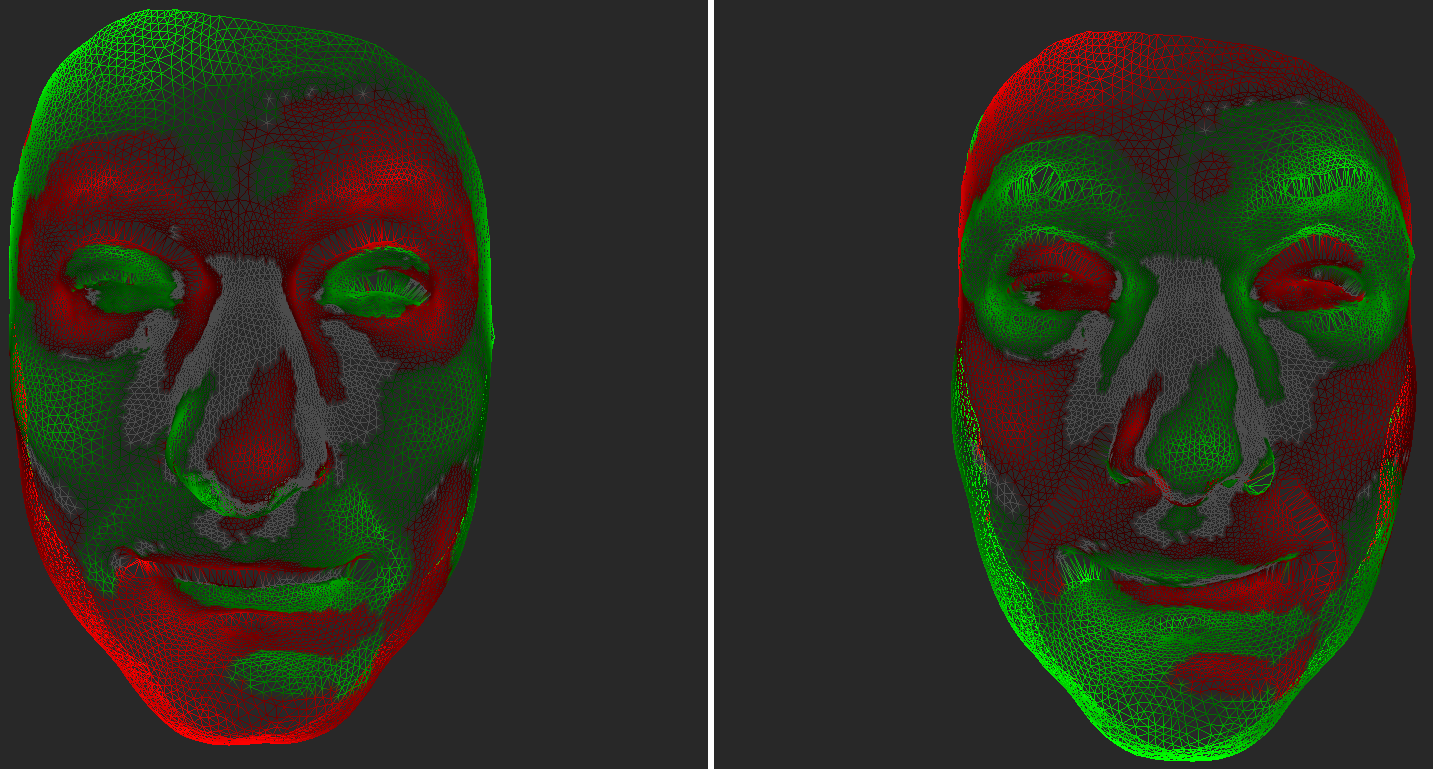
\includegraphics[width=\textwidth]{./screenshots/pair23.PNG}
\caption{}
\label{fig:8-23}
\end{subfigure}
\quad
\begin{subfigure}{0.4\textwidth}
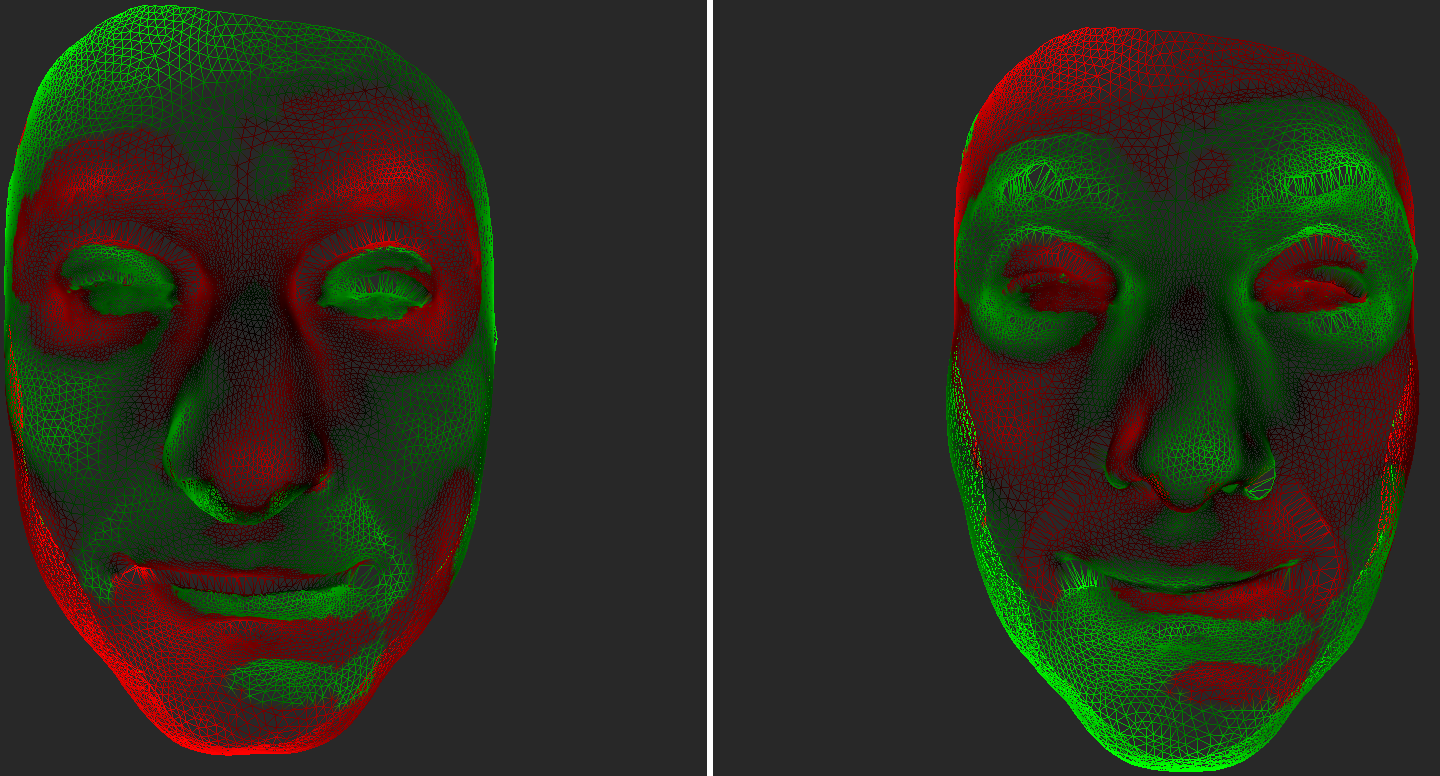
\includegraphics[width=\textwidth]{./screenshots/pair20.PNG}
\caption{}
\label{fig:8-20}
\end{subfigure}
\caption{Visualizations presented to the participants}
\end{figure}
\medskip
\begin{center}
\begin{tabular}{| c | c | c | c | c |}
	\hline
\multirow{2}{*}{\bf Answers} & \ref{fig:8-19} & \ref{fig:8-21} & \ref{fig:8-23} & \ref{fig:8-20}\\
	&  (\(t=47.23\)) &  (\(t=51.02\)) &  (\(t=36.77\)) &  (\(t=42.21\))\\ \hline
	NotSure & 2 & 1 & 1 & 2\\ \hline
	LeftCheek & 2 & 0 & 0 & 0\\ \hline
	Chin & 6 & 0 & 1 & 0\\ \hline
	RightCheek & 3 & 2 & 1 & 2\\ \hline
	Mouth & 0 & 2 & 1 & 0\\ \hline
	Nose & 0 & 5 & 3 & 1\\ \hline
	Forehead & 0 & 1 & 0 & 1\\ \hline
	{\bf Total} & {\bf 13} & {\bf 11} & {\bf 7} & {\bf 6}\\ \hline
\end{tabular}
\end{center}
\clearpage

\subsection{Question 10}

\begin{center}{\it When examining the differences moving from the left face to the right face, what is their main direction overall?}\end{center}

\begin{figure}[h]
\centering
\begin{subfigure}{0.4\textwidth}
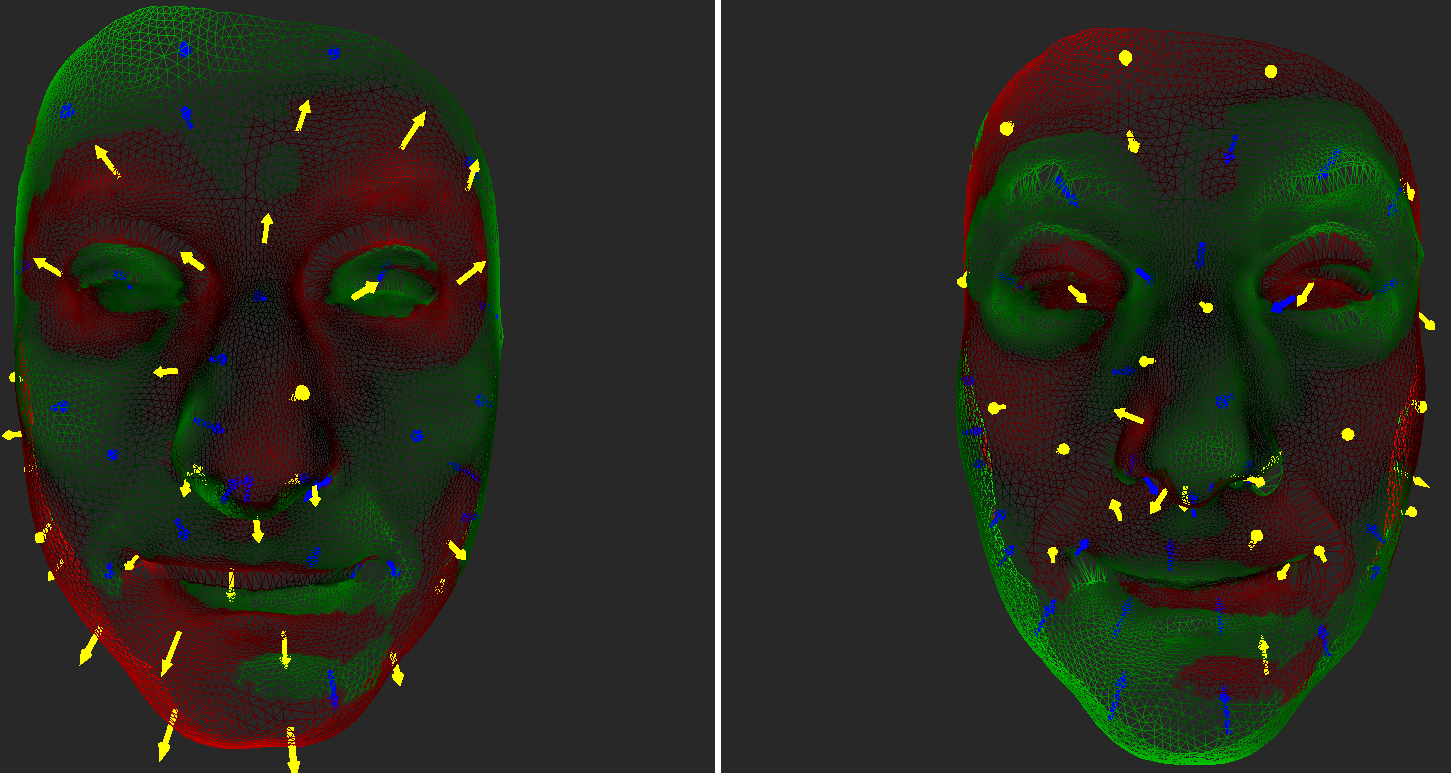
\includegraphics[width=\textwidth]{./screenshots/pair21.PNG}
\caption{}
\label{fig:9-21}
\end{subfigure}
\quad
\begin{subfigure}{0.4\textwidth}
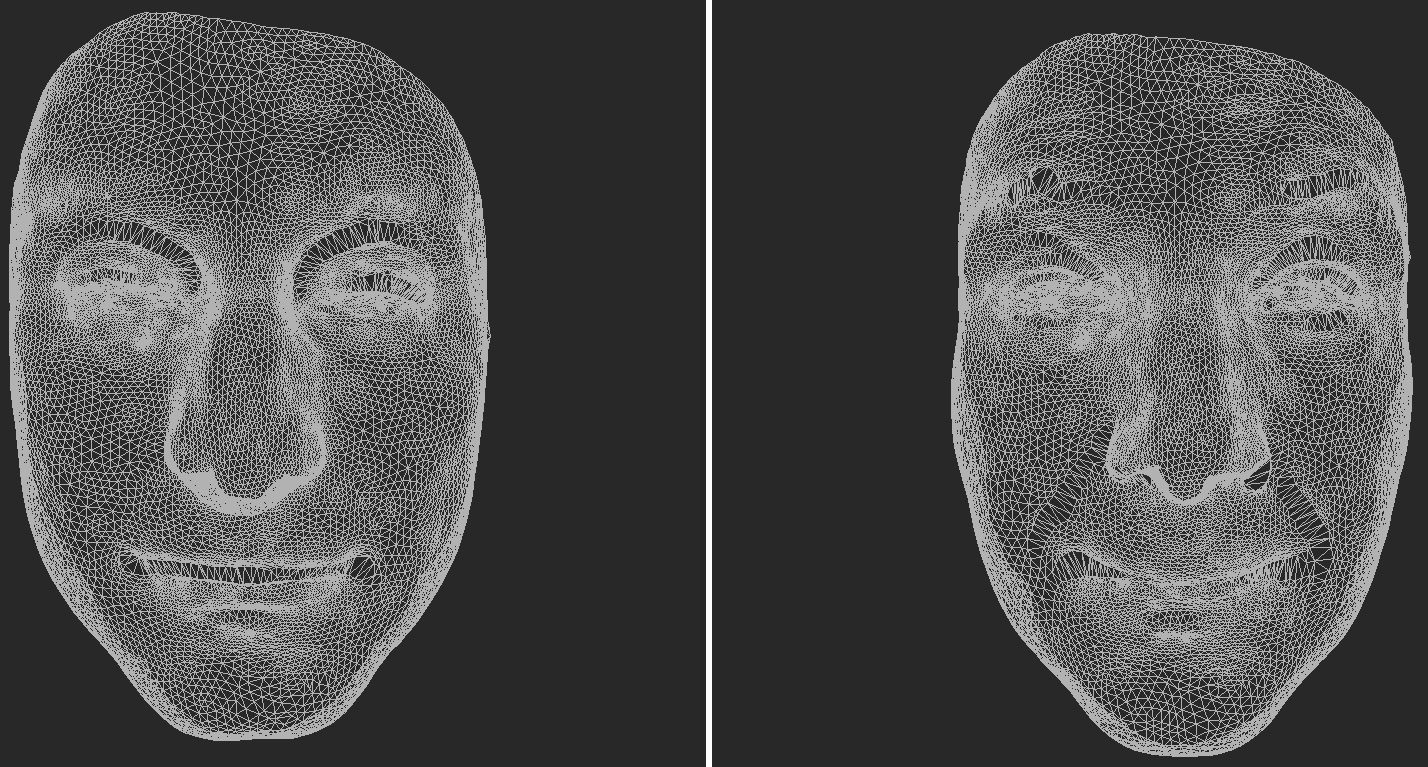
\includegraphics[width=\textwidth]{./screenshots/pair19.PNG}
\caption{}
\label{fig:9-19}
\end{subfigure}

\begin{subfigure}{0.4\textwidth}
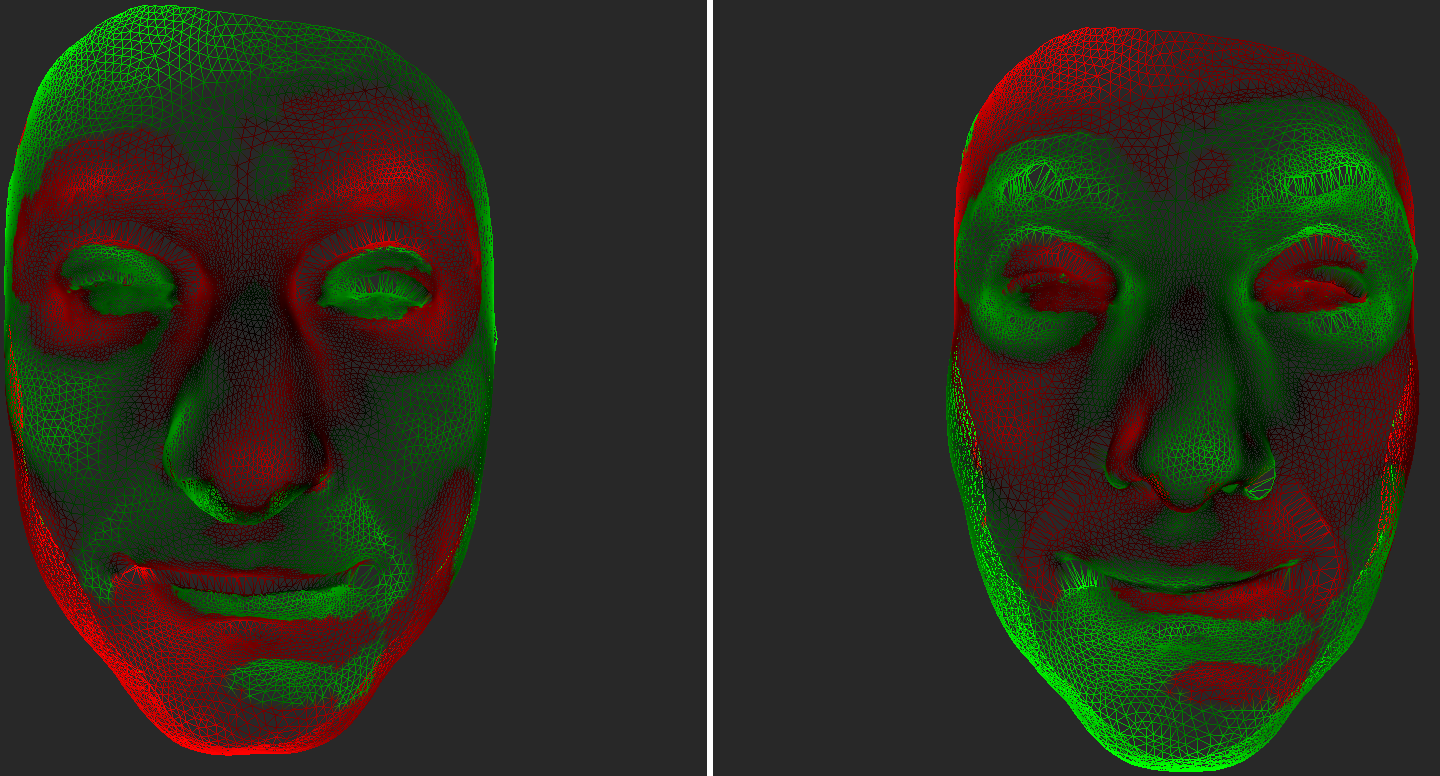
\includegraphics[width=\textwidth]{./screenshots/pair20.PNG}
\caption{}
\label{fig:9-20}
\end{subfigure}
\quad
\begin{subfigure}{0.4\textwidth}
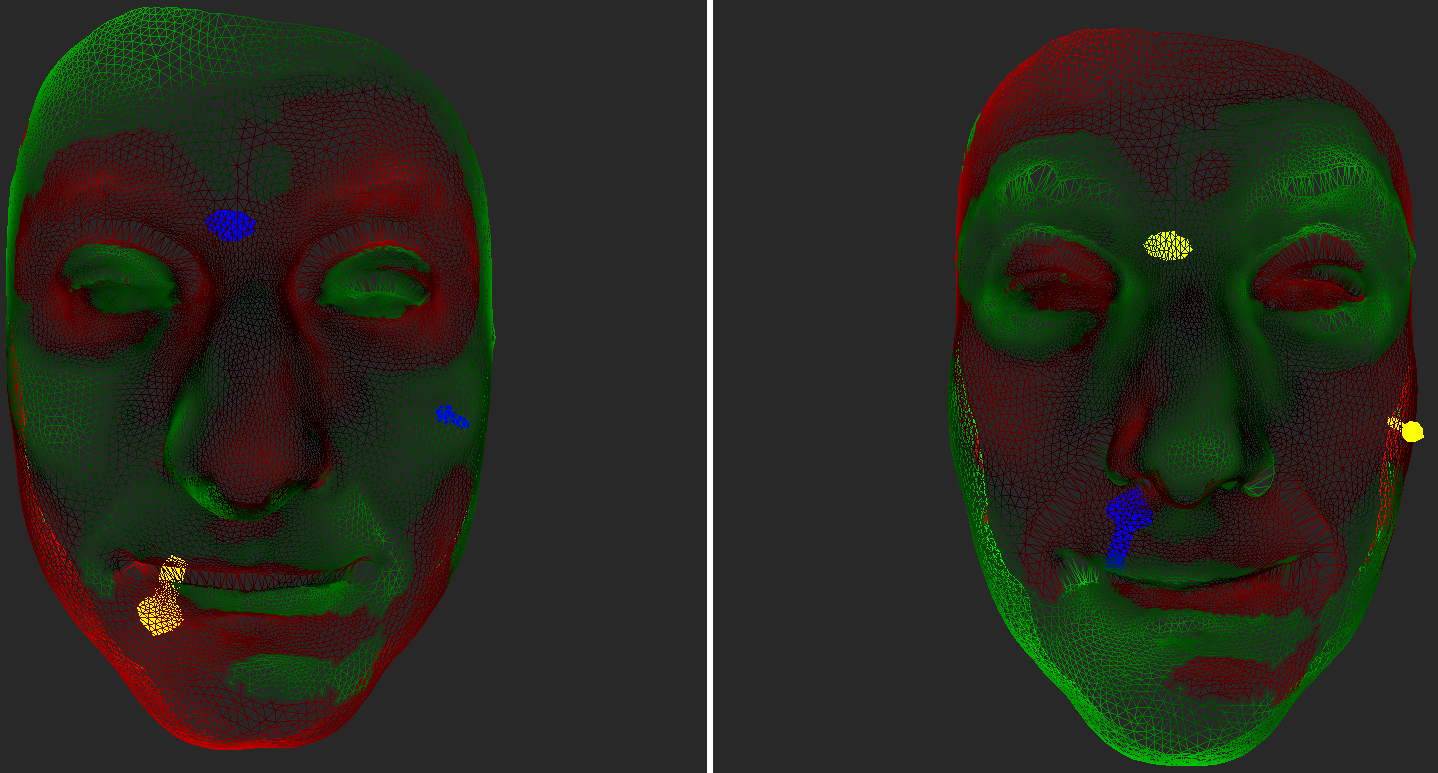
\includegraphics[width=\textwidth]{./screenshots/pair24.PNG}
\caption{}
\label{fig:9-24}
\end{subfigure}
\caption{Visualizations presented to the participants}
\end{figure}
\medskip
\begin{center}
\begin{tabular}{| c | c | c | c | c |}
	\hline
\multirow{2}{*}{\bf Answers} & \ref{fig:9-21} & \ref{fig:9-19} & \ref{fig:9-20} & \ref{fig:9-24}\\
	&  (\(t=50.42\)) &  (\(t=33.90\)) &  (\(t=48.06\)) &  (\(t=53.28\))\\ \hline
	NotSure & 4 & 2 & 2 & 1\\ \hline
	Down & 3 & 1 & 1 & 2\\ \hline
	In & 2 & 1 & 1 & 0\\ \hline
	Out & 3 & 4 & 2 & 0\\ \hline
	Up & 1 & 2 & 0 & 2\\ \hline
	Left & 0 & 1 & 0 & 0\\ \hline
	Right & 0 & 0 & 1 & 1\\ \hline
	{\bf Total} & {\bf 13} & {\bf 11} & {\bf 7} & {\bf 6}\\ \hline
\end{tabular}
\end{center}
\clearpage

